\documentclass[xcolor=pdftex,dvipsnames,table,mathserif]{beamer}
\usepackage{subfigure}
\usepackage{amsbsy}
\usepackage{tikz}
\usetikzlibrary{arrows}
\usepackage{amsmath,graphicx,dsfont,color}
\usepackage{amsfonts}
\usepackage{amssymb}
\usepackage{array}

\bibliographystyle{apalike}

\setbeamertemplate{bibliography item}{\insertbiblabel}
\setbeamertemplate{bibliography entry title}{}
\setbeamertemplate{bibliography entry location}{}
\setbeamertemplate{bibliography entry note}{}

%Definitiona

\newcommand{\x}{\mathbf{x}}
\newcommand{\X}{\mathbf{X}}
\newcommand{\W}{\mathbf{W}} %Weight
\newcommand{\bais}{\mathbf{b}}%Bais
\newcommand{\act}{\texttt{g}}%Activation
\newcommand{\loss}{L}
\newcommand{\pdata}{\hat{p}_{\texttt{data}}}
\newcommand{\nsize}{n}
\newcommand{\param}{\boldsymbol{\theta}}
\newcommand{\featmap}{\boldsymbol{\phi}}
\newcommand{\EV}{\mathbb{E}}







\usepackage{physics}
\usepackage{tikz}
\usetikzlibrary{fit,positioning}
%\setbeamercovered{transparent}

\graphicspath{{../graphics/}}

\AtBeginSection[]{
  \begin{frame}{Contents}
    \tableofcontents[currentsection, hideothersubsections]
  \end{frame}
}

\AtBeginSubsection[]{
  \begin{frame}{Contents}
    \tableofcontents[currentsection, subsectionstyle=show/shaded/hide]
  \end{frame}
}

\setbeamertemplate{footline}[frame number]{}
\setbeamertemplate{navigation symbols}{}
\setbeamertemplate{section in toc}[square]
\setbeamertemplate{items}[square]

%% For image credits on image bottom right
\usepackage[absolute,overlay]{textpos}
\setbeamercolor{framesource}{fg=gray}
\setbeamerfont{framesource}{size=\tiny}
\newcommand{\source}[1]{\begin{textblock*}{4cm}(8.7cm,8.6cm)
    \begin{beamercolorbox}[ht=0.5cm,right]{framesource}
      \usebeamerfont{framesource}\usebeamercolor[fg]{framesource} Credits: {#1}
    \end{beamercolorbox}
\end{textblock*}}

\title{Deep learning for image analysis quick introduction}
\author{E. Decencière}
\date{MINES ParisTech\\
  PSL Research University\\
  Center for Mathematical Morphology
}
\titlegraphic{
\includegraphics[height=1.7cm]{../graphics/logoemp}}

\useinnertheme{rounded}
\usecolortheme{rose}

%%%%%%%%%%%%%%%%%%%%%%%%%%%%%%%%%%%%%%%%%%%%%%%%%%%%%%%
%%%%%%%%%%%%%%%%%%%%%%%%%%%%%%%%%%%%%%%%%%%%%%%%%%%%%%%

\begin{document}

\frame{\titlepage}

\frame{
  \frametitle{Contents}
  \tableofcontents[hidesubsections]
}

%%%%%%%%%%%%%%%%%%%%%%%%%%%%%%%%%%%%%%%%%%%%%%%%%%
%%%%%%%%%%%%%%%%%%%%%%%%%%%%%%%%%%%%%%%%%%%%%%%%%%
\section{Introduction}

%%%%%%%%%%%%%%%%%%%%%%%%%%%%%%%%%%%%
\begin{frame}{The rise of deep learning}

\begin{figure}[ht]
  \centering
  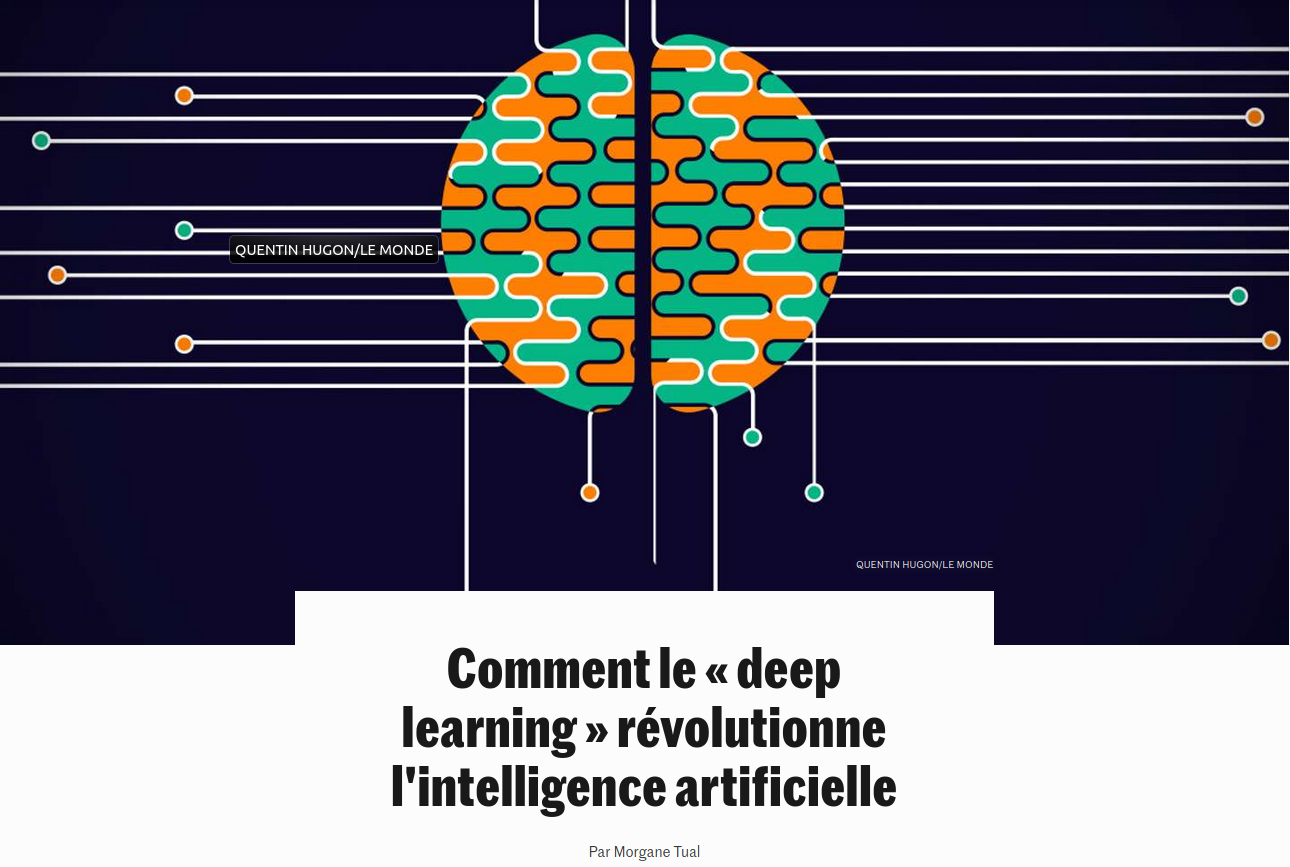
\includegraphics[height=0.5\textheight]{lemonde-juillet2015}
  \caption*{Le Monde, juillet 2015}
\end{figure}


\end{frame}

%%%%%%%%%%%%%%%%%%%%%%%%%%%%%%%%%%%%
\begin{frame}{The rise of deep learning}

\begin{figure}[ht]
  \centering
  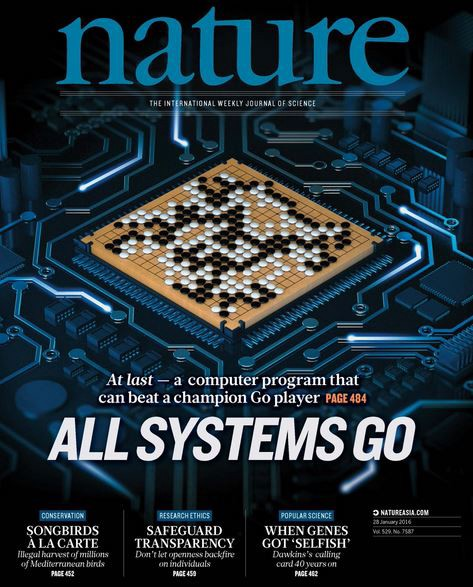
\includegraphics[height=0.5\textheight]{nature_go}
  \caption*{Nature, 2016}
\end{figure}


\end{frame}


%%%%%%%%%%%%%%%%%%%%%%%%%%%%%%%%%%%%
\begin{frame}{The rise of deep learning}

\begin{figure}[ht]
  \centering
  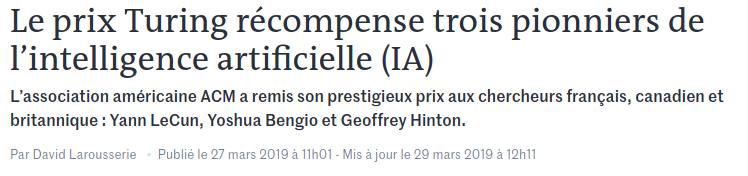
\includegraphics[width=0.7\textwidth]{lemonde27mars2019}
  \caption*{Le Monde, mars 2019}
\end{figure}


\end{frame}

%%%%%%%%%%%%%%%%%%%%%%%%%%%%%%%%%%%%
\begin{frame}{The rise of deep learning}


\begin{figure}[ht]
  \centering
  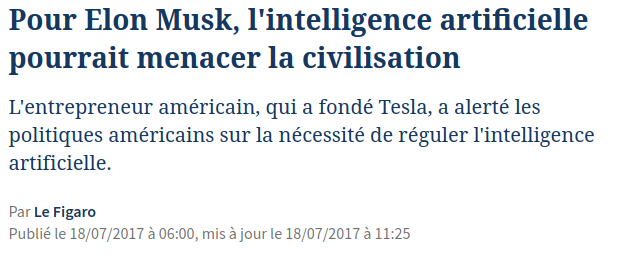
\includegraphics[width=0.7\textwidth]{le_figaro_musk}
  \caption*{Le Figaro, juillet 2017}
\end{figure}



\end{frame}


%%%%%%%%%%%%%%%%%%%%%%%%%%%%%%%%%%%%%%%%%%%%%%%%%%
\section{Artificial neural networks}
%%%%%%%%%%%%%%%%%%%%%%%%%%%%%%%%%%%%%%%%%%%%%%%%%%

%%%%%%%%%%%%%%%%%%%%%%%%%%%%%%%%%%%%%%%%%%%%%%%%%%
\frame{
\frametitle{Artificial neural networks and deep learning history}


%% \begin{block}{}
%%   For a very complete state of the art on deep learning, see the overview by Schmidhuber \cite{schmidhuber_deep_2015}.
%% \end{block}

\begin{itemize}[<+->]
\item 1958: Perceptron {\tiny\cite{rosenblatt_perceptron:_1958}}.
\item 1979: Convolutional neural networks {\tiny\cite{fukushima_neural_1979}}.
\item 1980's: Backpropagation algorithm {\tiny\cite{werbos_applications_1982,lecun_procedure_1985}}.
\item 2006-: Implementations on Graphical Processing Units
\item 2012: Imagenet image classification won by a convolutional neural network {\tiny\cite{krizhevsky_imagenet_2012}}.

\end{itemize}

}



%%%%%%%%%%%%%%%%%%%%%%%%%%%%%%%%%%%%
\begin{frame}{Artificial neuron}

    \begin{figure}
      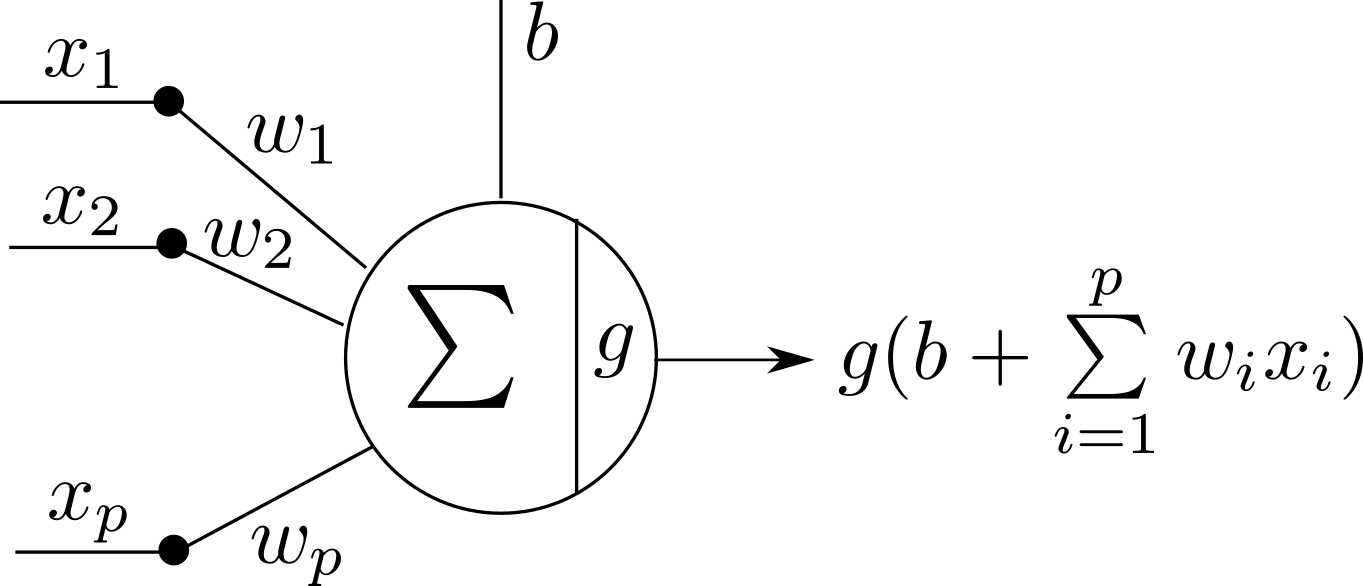
\includegraphics[height=3cm]{neurone_representation_compacte}
    \end{figure}

\end{frame}


%%%%%%%%%%%%%%%%%%%%%%%%%%%%%%%%%%%%%%%%%%%%%%%%%%

\frame{
  \frametitle{Activation: rectified linear unit (ReLU)}

  \begin{columns}
    \begin{column}{.5\textwidth}
      \[
      \act(x)=
      \begin{cases}
        x,& \text{if } x > 0\\
        0,              & \text{otherwise}
      \end{cases}
      \]
    \end{column}

    \begin{column}{.5\textwidth}
      \begin{figure}
        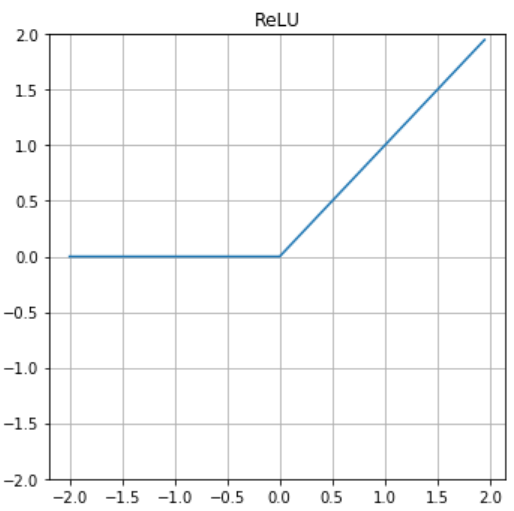
\includegraphics[width=.8\textwidth]{act_relu.png}
      \end{figure}


    \end{column}
  \end{columns}

  \begin{block}{Remarks}
    \begin{itemize}
    \item[+] Usable gradient when activated
    \item[+] Fast to compute
    \item[+] High abstraction
    \end{itemize}
  \end{block}

\pause

  \begin{alertblock}{}
    ReLU is the most commonly used activation function.
  \end{alertblock}


}

%%%%%%%%%%%%%%%%%%%%%%%%%%%%%%%%%%%%%%%%%%%%%%%%%%

\frame{
  \frametitle{What can an artificial neuron compute?}

  \begin{figure}
    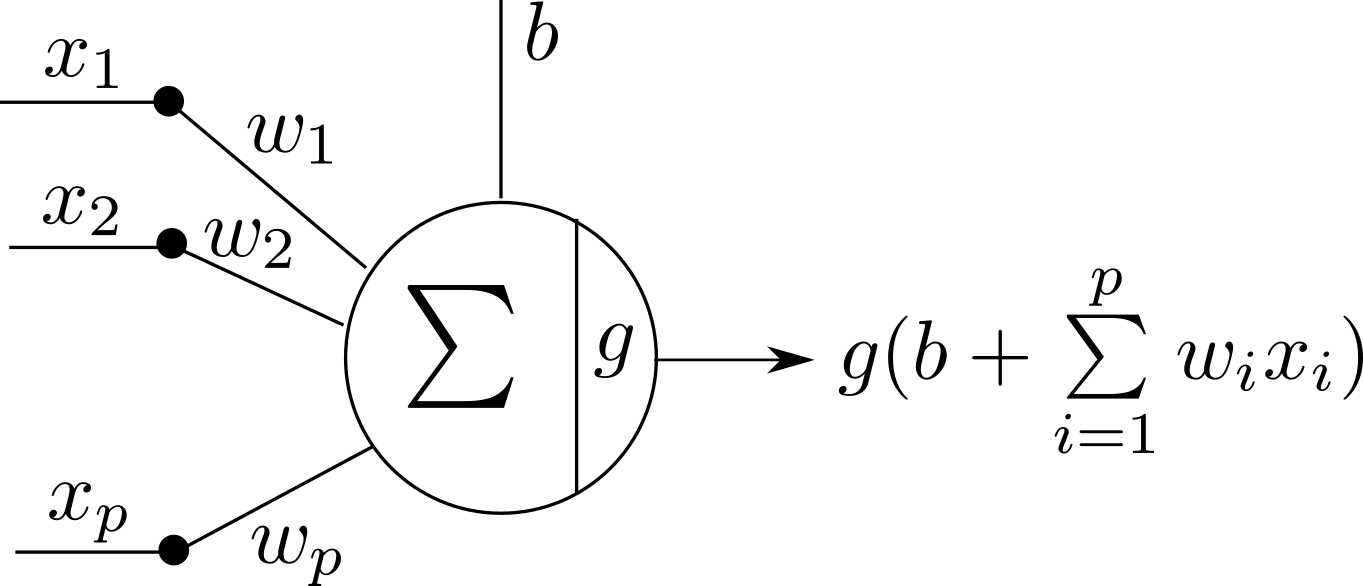
\includegraphics[height=3cm]{neurone_representation_compacte}
  \end{figure}

  \begin{block}{}
    In $\R^p$ ,
    $b + \sum\limits_{i=1}^p w_ix_i = 0$
    corresponds to a hyperplane $H$. For a given point
    $\x = \{x_1, \ldots, x_p\}$,
    decisions are made according to the side of the hyperplane it belongs to.
  \end{block}

  %% \begin{alertblock}{}
  %%   When the activation function is binary, we obtain a \alert{perceptron}
  %% \end{alertblock}

}

%%%%%%%%%%%%%%%%%%%%%%%%%%%%%%%%%%%%%%%%%%%%%%%%%%

\frame{
  \frametitle{Example}

  \begin{figure}
    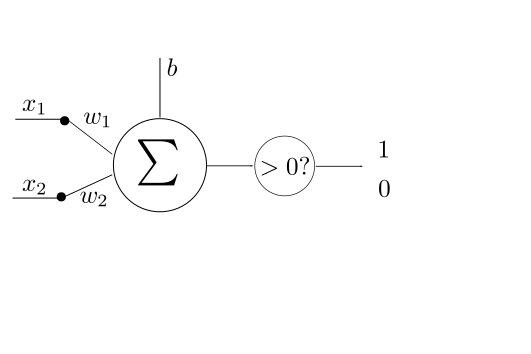
\includegraphics[height=3cm]{neurone_simple}
  \end{figure}

  \begin{itemize}
  \item $p=2$ : 2-dimensional inputs (can be represented on a screen!)
  \item Activation: binary
  \item Classification problem
  \end{itemize}
}

%%%%%%%%%%%%%%%%%%%%%%%%%%%%%%%%%%%%%%%%%%%%%%%%%%

\frame{
  \frametitle{Gaussian clouds}

  \begin{figure}
    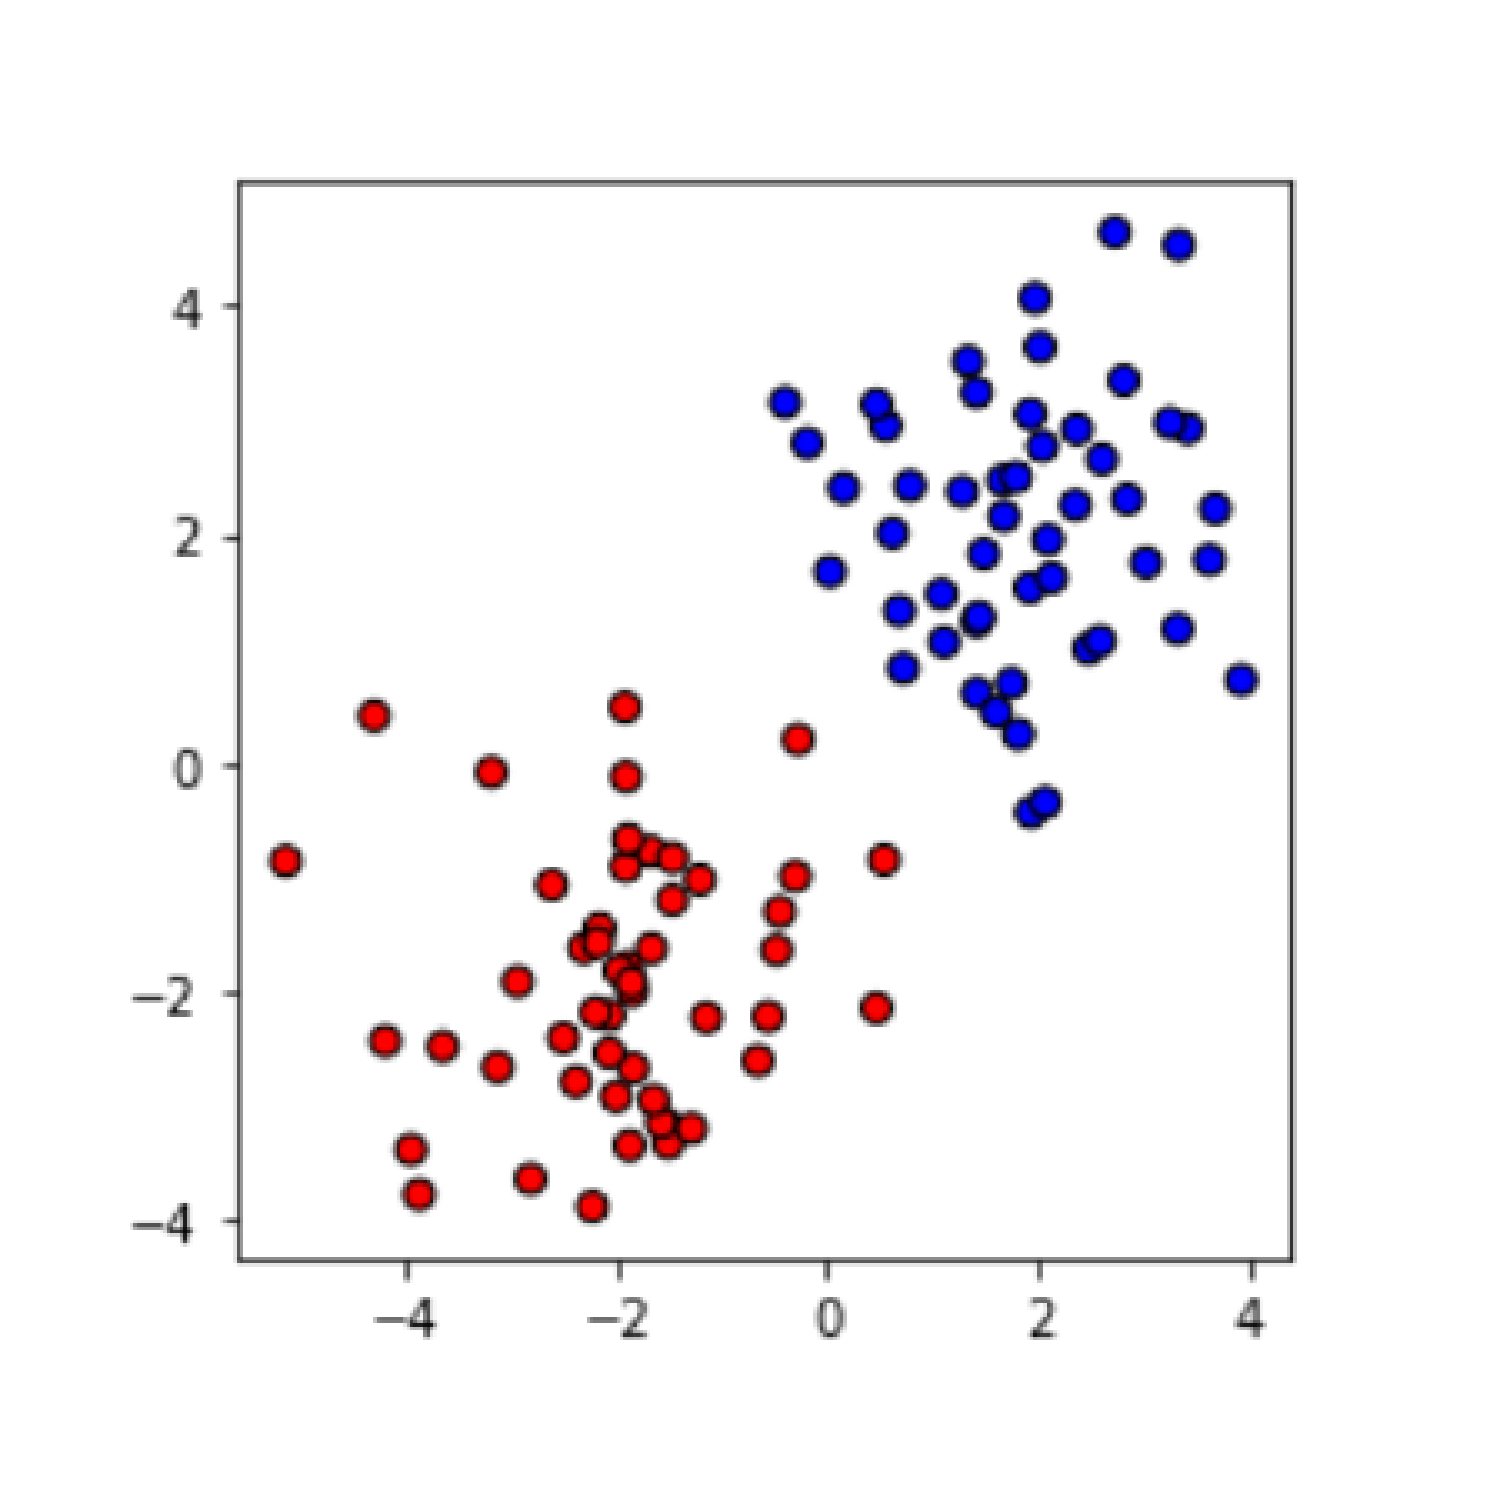
\includegraphics[height=6cm]{gaussian_clouds}
  \end{figure}


}

%%%%%%%%%%%%%%%%%%%%%%%%%%%%%%%%%%%%%%%%%%%%%%%%%%

\frame{
  \frametitle{Gaussian clouds}

  \begin{figure}
    \includegraphics[height=6cm]{gaussian_clouds_H}
  \end{figure}


}

%%%%%%%%%%%%%%%%%%%%%%%%%%%%%%%%%%%%%%%%%%%%%%%%%%

\frame{
  \frametitle{Circles}

  \begin{figure}
    \includegraphics[height=6cm]{circles}
  \end{figure}


}

%%%%%%%%%%%%%%%%%%%%%%%%%%%%%%%%%%%%%%%%%%%%%%%%%%

%% \frame<beamer>{
%%   \frametitle{Solution?}

%%   \begin{figure}
%%     \includegraphics[height=3cm]{circles}
%%   \end{figure}

%% \begin{itemize}
%%    \item Transform the input space, for example use a polar transformation
%%    \item Increase the number of input dimensions: for example add $x_1^2, x_2^2, x_1 x_2$ to the initial features $x_1, x_2$
%%    \item Combine several neurons
%% \end{itemize}

%% }



%%%%%%%%%%%%%%%%%%%%%%%%%%%%%%%%%%%%%%%%%%%%%%%%%%

\frame{
  \frametitle{Circles}

  \begin{figure}
    \includegraphics[height=6cm]{circles_H}
  \end{figure}

\begin{block}{Playing with artificial neural networks}
  \url{https://playground.tensorflow.org}
\end{block}

}

%%%%%%%%%%%%%%%%%%%%%%%%%%%%%%%%%%%%%%%%%%%%%%%%%%

\frame{
  \frametitle{Solution}

  \begin{columns}
    \begin{column}{.5\textwidth}
      \begin{figure}
        \includegraphics[height=5cm]{ann_5}
      \end{figure}

    \end{column}

    \begin{column}{.5\textwidth}

      \begin{figure}
        \includegraphics[height=4cm]{circles_H}
      \end{figure}

    \end{column}
  \end{columns}

  \begin{block}{Universal approximation theorem \cite{cybenko_approximations_1989,hornik_approximation_1991}}
    Any continuous real-valued function of $[0,1]^p$ can be approximated by an artificial neural network with a single hidden layer.
  \end{block}

}

%%%%%%%%%%%%%%%%%%%%%%%%%%%%%%%%%%%%%%%%%%%%%%%%%%
\frame{
\frametitle{Multi-layered perceptron}

\begin{figure}
  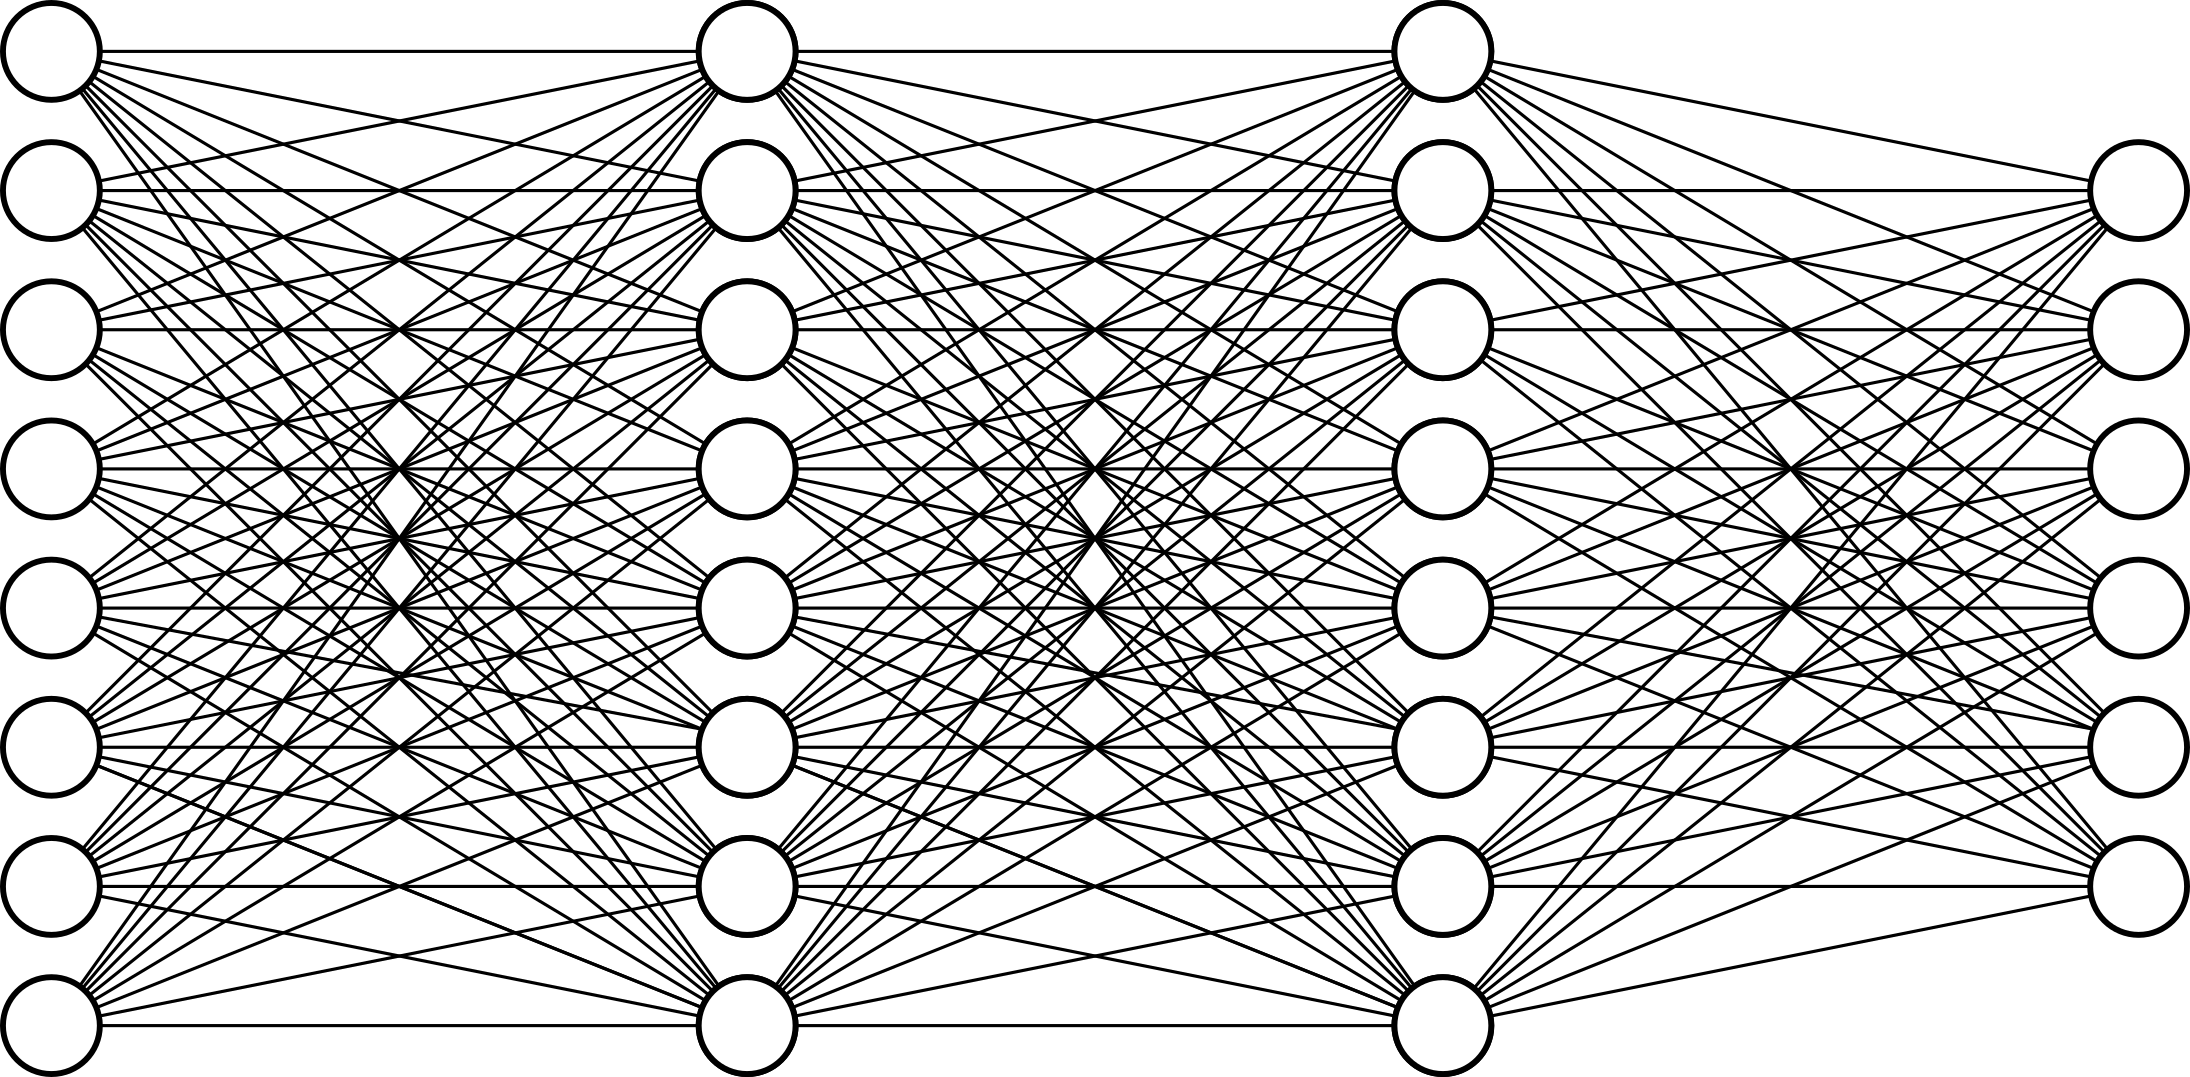
\includegraphics[height=3cm]{mini_reseau3_bis.png}
\end{figure}

\begin{alertblock}{Deep learning}<2->
  \begin{itemize}
  \item<2-> Artificial neural networks with \textit{many} layers.
  \item<3-> Features get more specific with depth
  \end{itemize}

\end{alertblock}

}

%%%%%%%%%%%%%%%%%%%%%%%%%%%%%%%%%%%%
\begin{frame}{Graphical representation of NNs}

\begin{columns}
  \begin{column}{.5\textwidth}
    \begin{figure}
      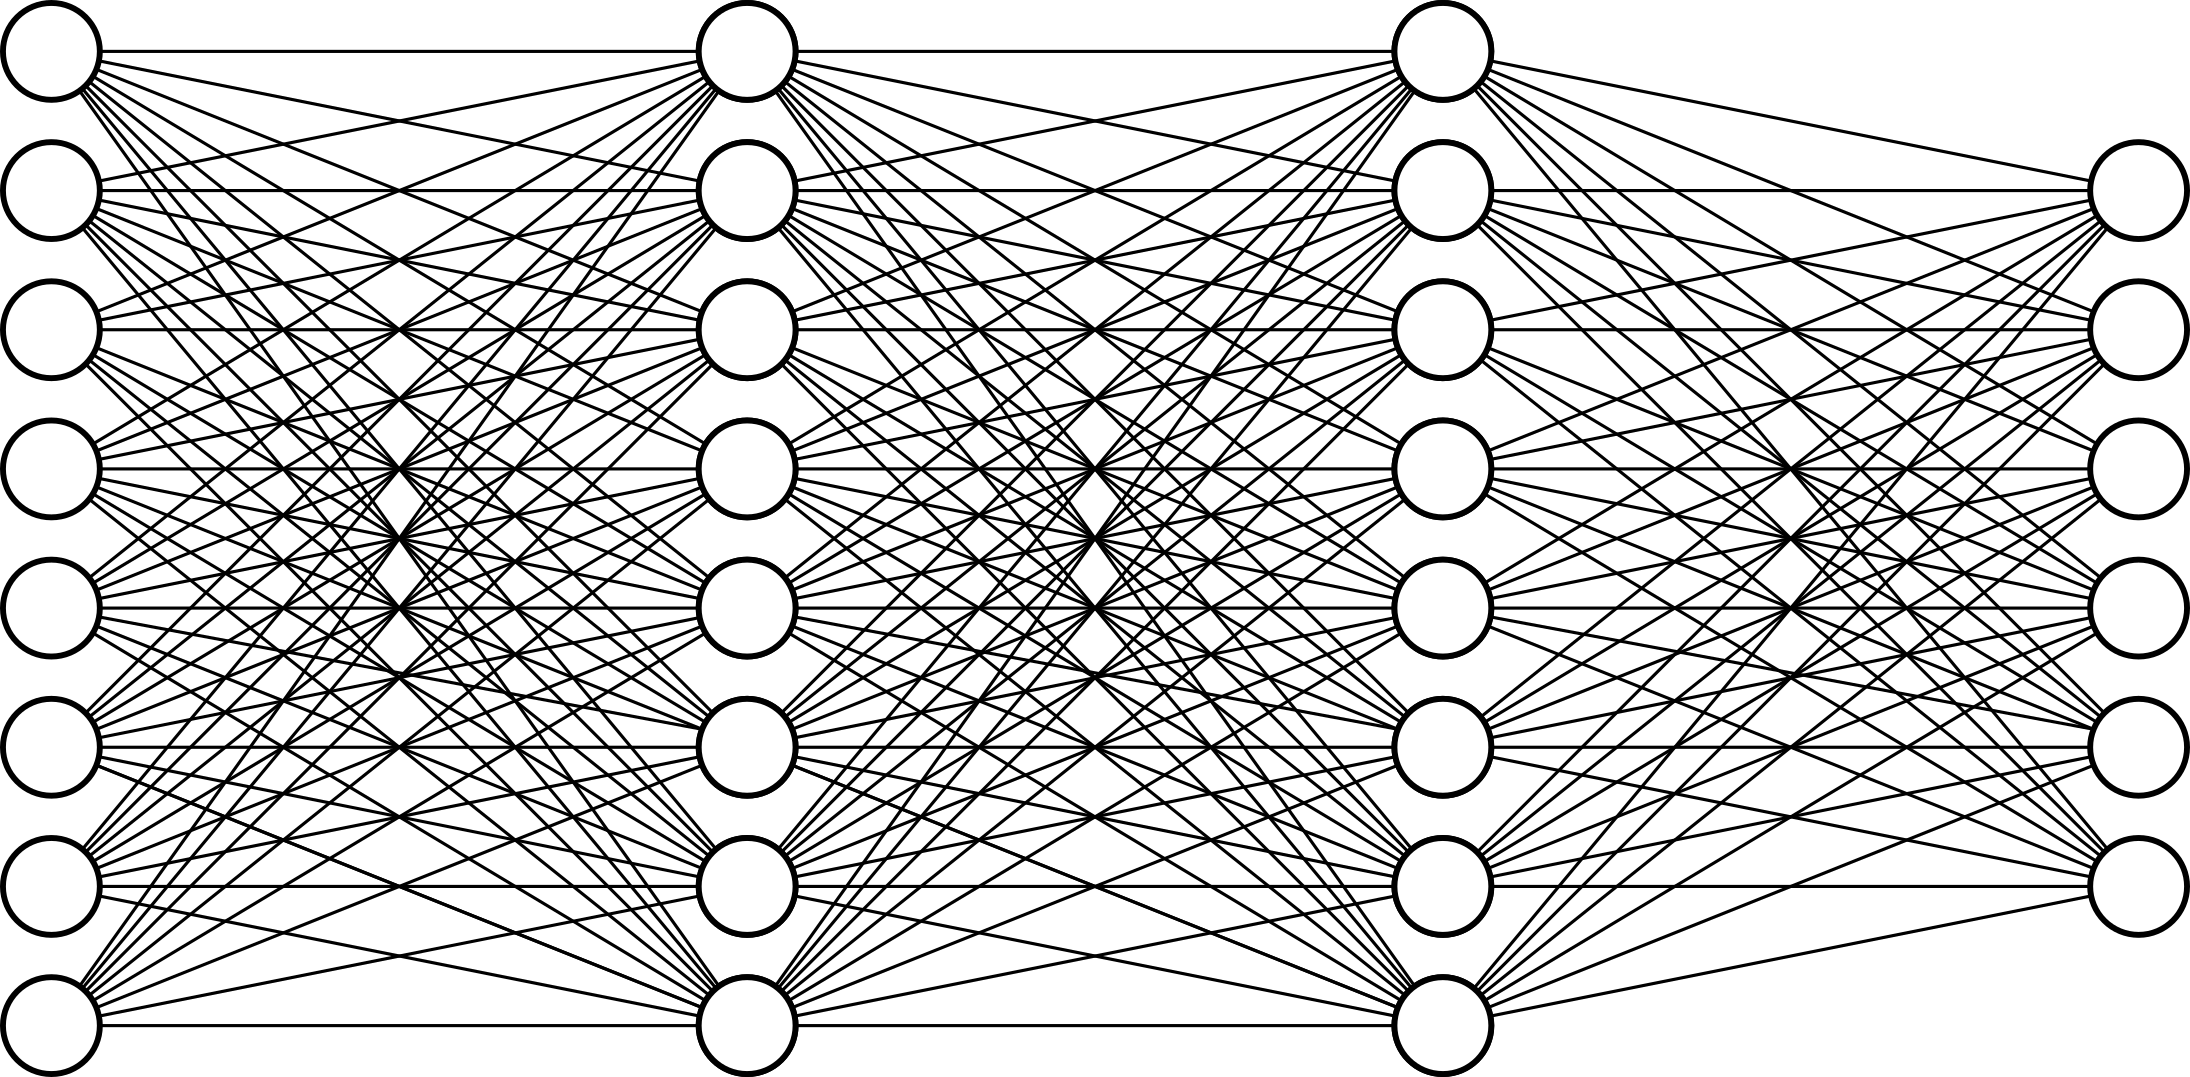
\includegraphics[height=3cm]{mini_reseau3_bis.png}
    \end{figure}
    \begin{figure}
      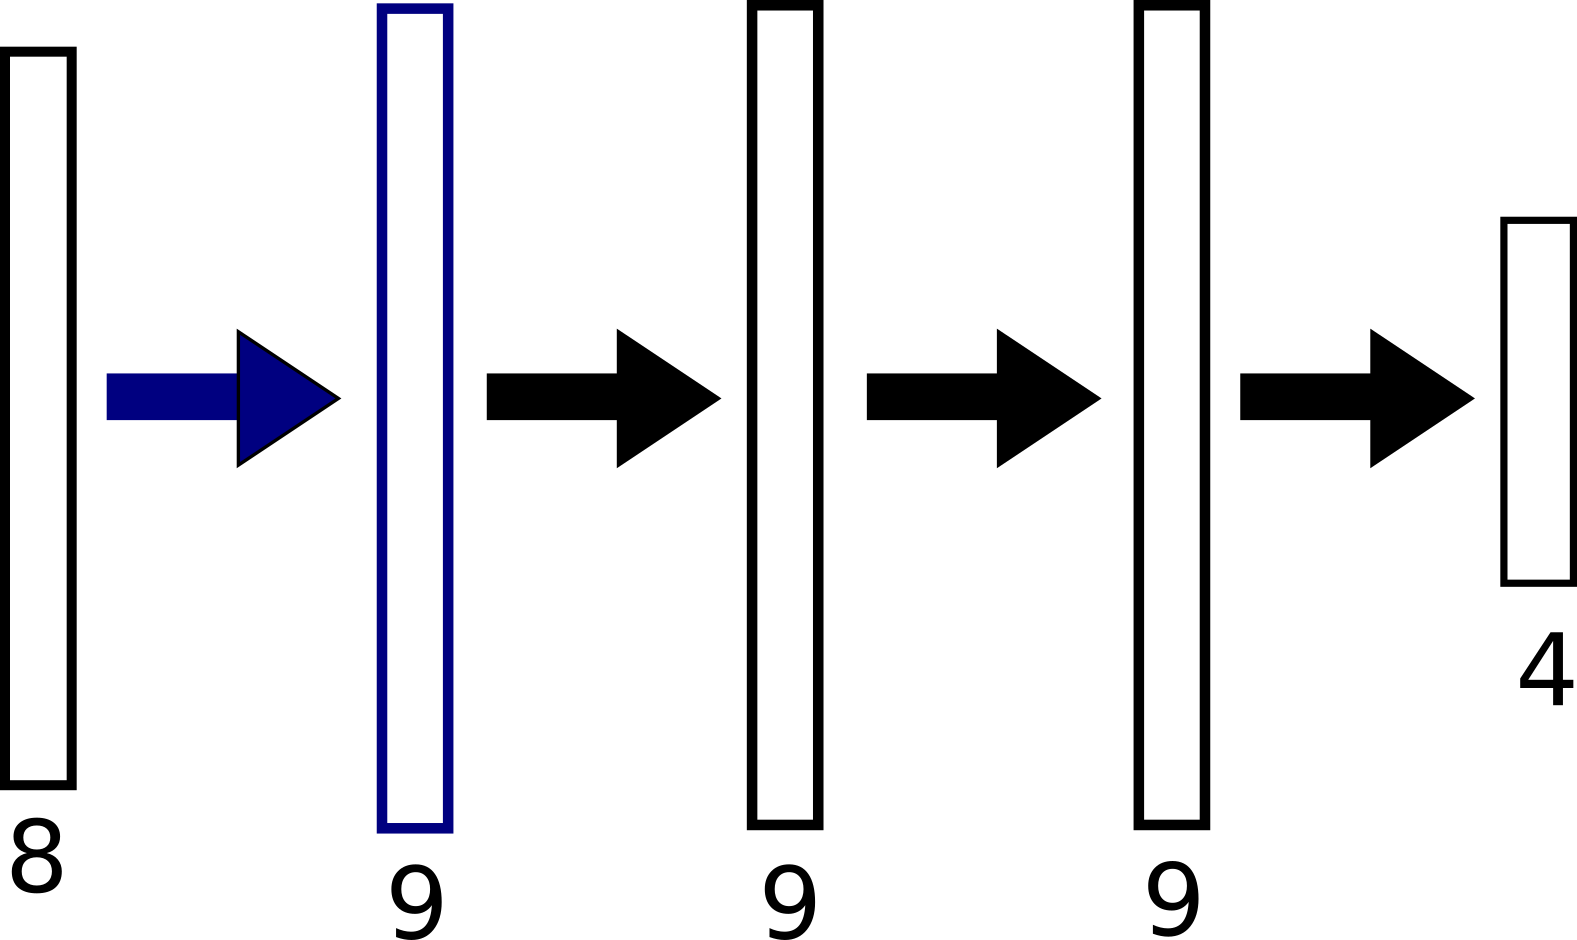
\includegraphics[height=3cm]{nn_representation}
    \end{figure}
  \end{column}

  \begin{column}{.5\textwidth}
    \begin{itemize}
    \item Data is organized into arrays, linked with operators
    \item A layer corresponds to an operator between arrays.
    \end{itemize}
  \end{column}
\end{columns}

\end{frame}


%%%%%%%%%%%%%%%%%%%%%%%%%%%%%%%%%%%%
\begin{frame}{Learning with artificial neural networks}

\begin{itemize}
\item Constitute your learning, validation and test sets
\item Define a loss function
\item Use gradient descent (backpropagation) to minimize the loss
\end{itemize}

\end{frame}


%%%%%%%%%%%%%%%%%%%%%%%%%%%%%%%%%%%%
\section{Application to images}

%%%%%%%%%%%%%%%%%%%%%%%%%%%%%%%%%%%%
\begin{frame}{A picture is worth a thousand words}


      \begin{figure}
        \centering
        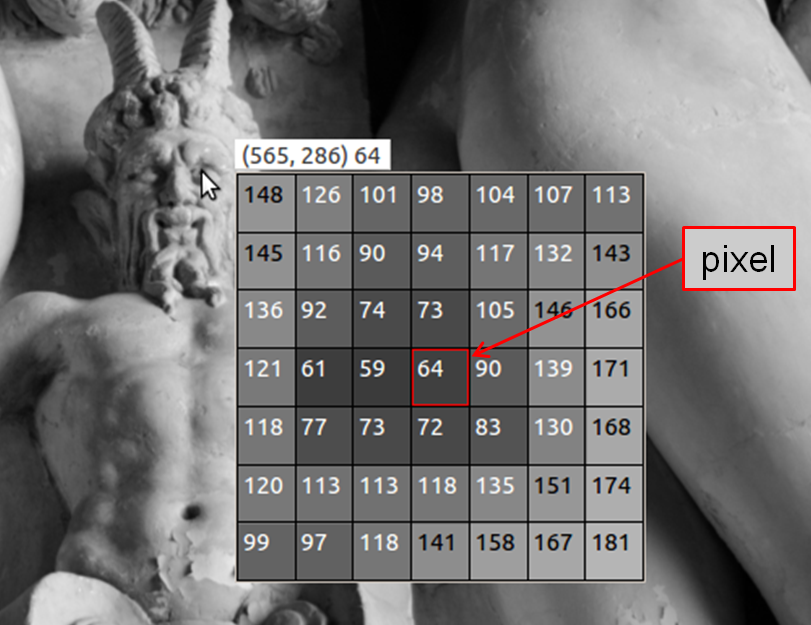
\includegraphics[width=6cm]{faune.png}\\
        \tiny{Grey level values around the left eye of the faun}
      \end{figure}

      \begin{itemize}
      \item<2-> Deep learning excels in image analysis.
      \end{itemize}

\end{frame}


%%%%%%%%%%%%%%%%%%%%%%%%%%%%%%%%%%%%
\begin{frame}{The role of annotated image databases}

  Image databases including \emph{annotations} (typically some kind of high level information) are essential to the development of \emph{supervised} machine learning methods for image analysis.

  \begin{block}{Annotations}
    \begin{itemize}
    \item Image class
    \item Measure(s) obtained from the image
    \item Position of objects within the image
    \item Segmentation
    \end{itemize}
  \end{block}

\end{frame}

%%%%%%%%%%%%%%%%%%%%%%%%%%%%%%%%%%%%
%% \begin{frame}{MNIST database \tiny{\cite{lecun_gradient-based_1998}}}

%%   \begin{itemize}
%%   \item The Modified National Institute of Standards and Technology (MNIST) database contains $60\,000$ training images of hand-written digits, and $10,000$ test images.
%%   \item Image size: $28 \times 28$
%%   \end{itemize}

%%   \centering
%%   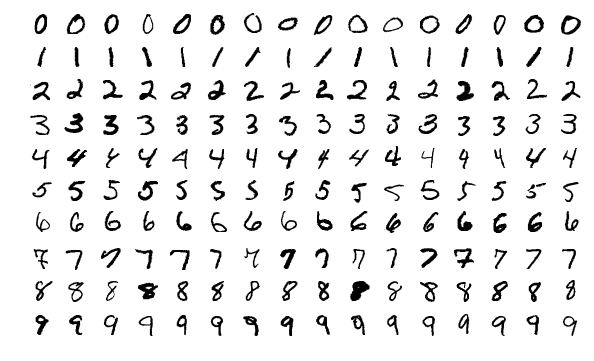
\includegraphics[width=0.75\textwidth]{mnist_examples.png}\\
%%   \source{Images from MNIST assembled by Josef Stepan (licensed under CC BY-SA 4.0)}

%% \end{frame}


%%%%%%%%%%%%%%%%%%%%%%%%%%%%%%%%%%%%
\begin{frame}{PatchCamelyon database}

\begin{figure}[ht]
  \centering
  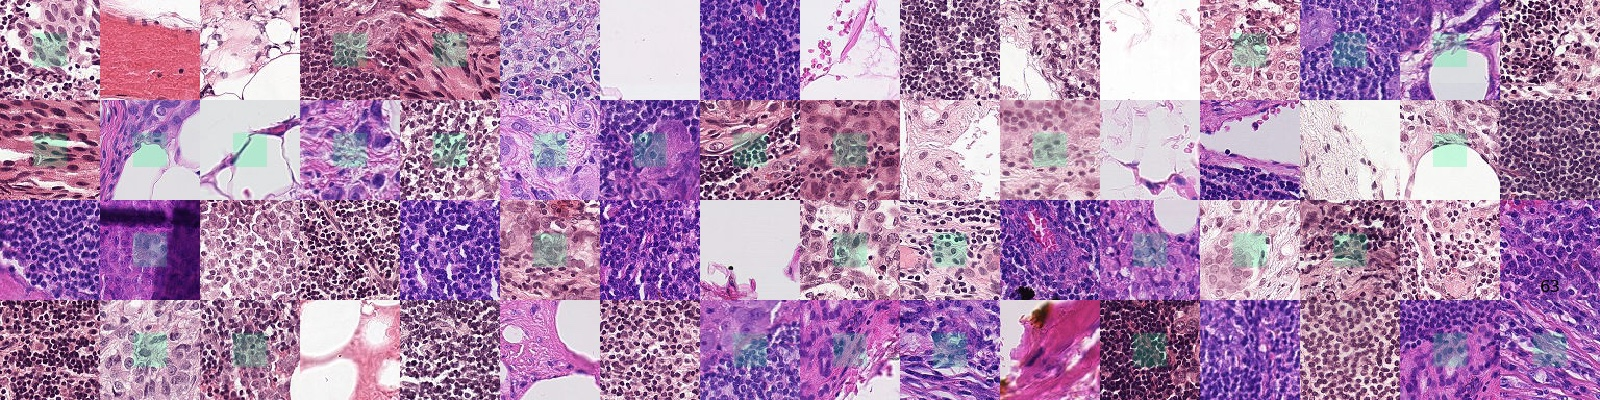
\includegraphics[width=\textwidth]{pcam.jpg}
\end{figure}

\begin{itemize}
\item $327\,680$ images of size $96 \times 96$
\item Binary label (tumor tissue in center region or not)
\item \url{https://github.com/basveeling/pcam}
\end{itemize}

\end{frame}


%%%%%%%%%%%%%%%%%%%%%%%%%%%%%%%%%%%%
\begin{frame}{Layers representation}

  %% \begin{block}{}
  %%   For illustration purposes, in the following slides images and filters will be displayed as rows of neurons -- these can be seen as 1D arrays or as sections of 2D arrays.

  %%   We represent some connections between neurons. Each such connection is associated to a weight. The bias are not represented, to avoid clutter, but must not be forgotten.
  %% \end{block}

  \begin{columns}

    \begin{column}<1->{0.33\textwidth}
      \begin{center}
        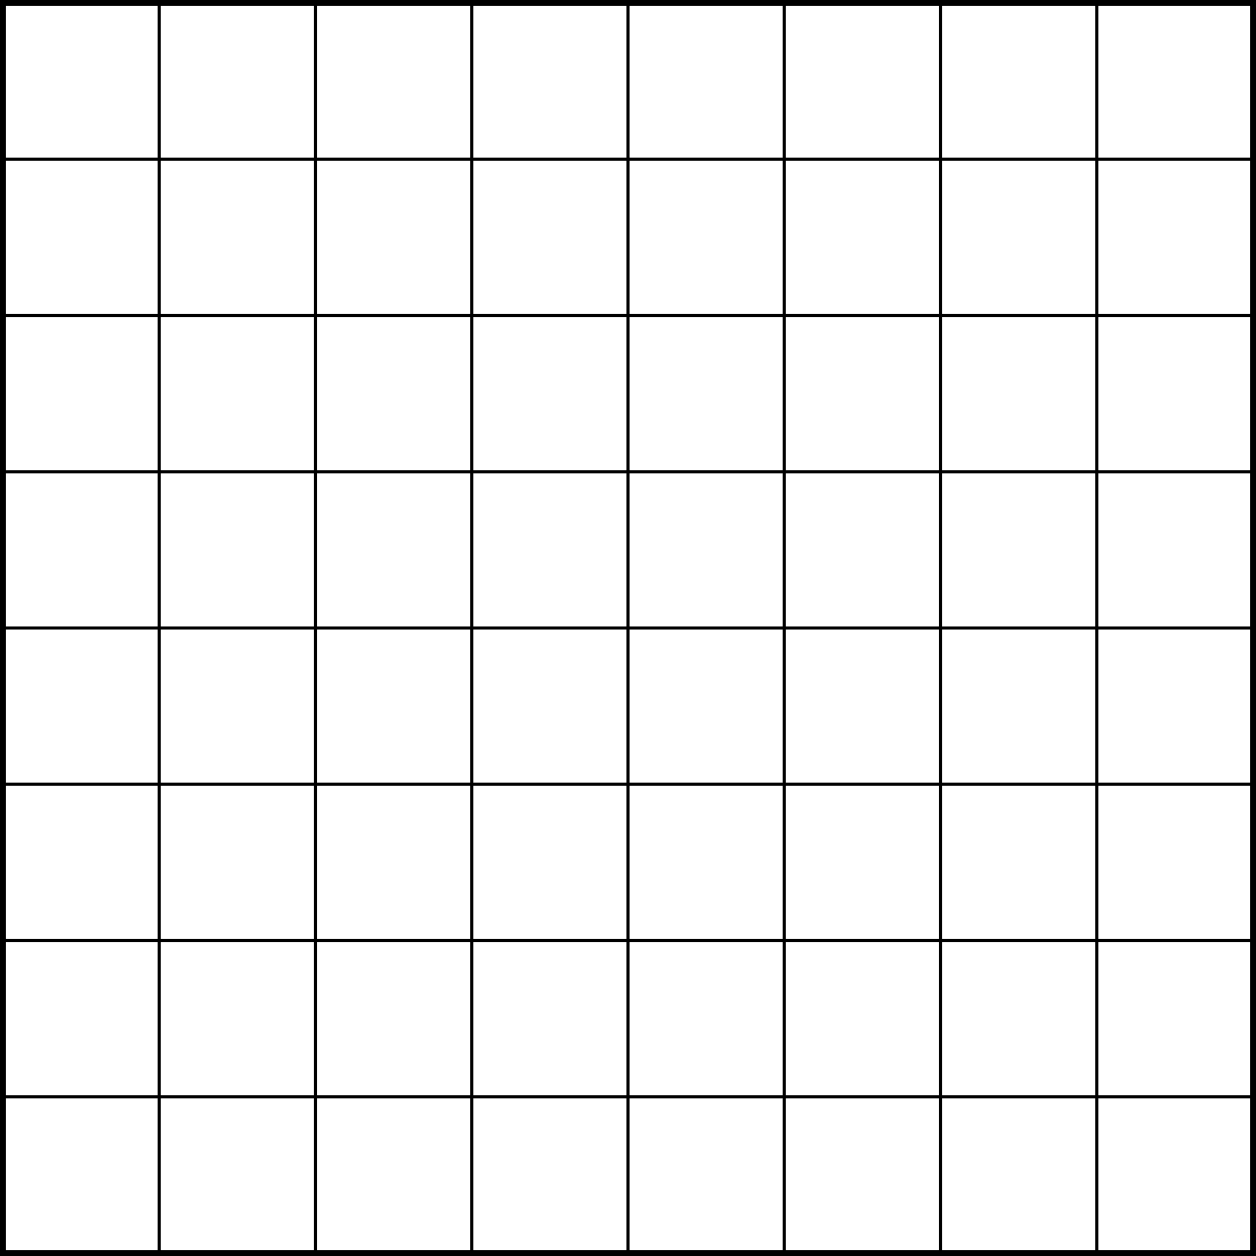
\includegraphics[width=0.80\textwidth]{cnn_pixels.png}
      \end{center}
    \end{column}

    \begin{column}<2->{0.33\textwidth}
      \begin{center}
        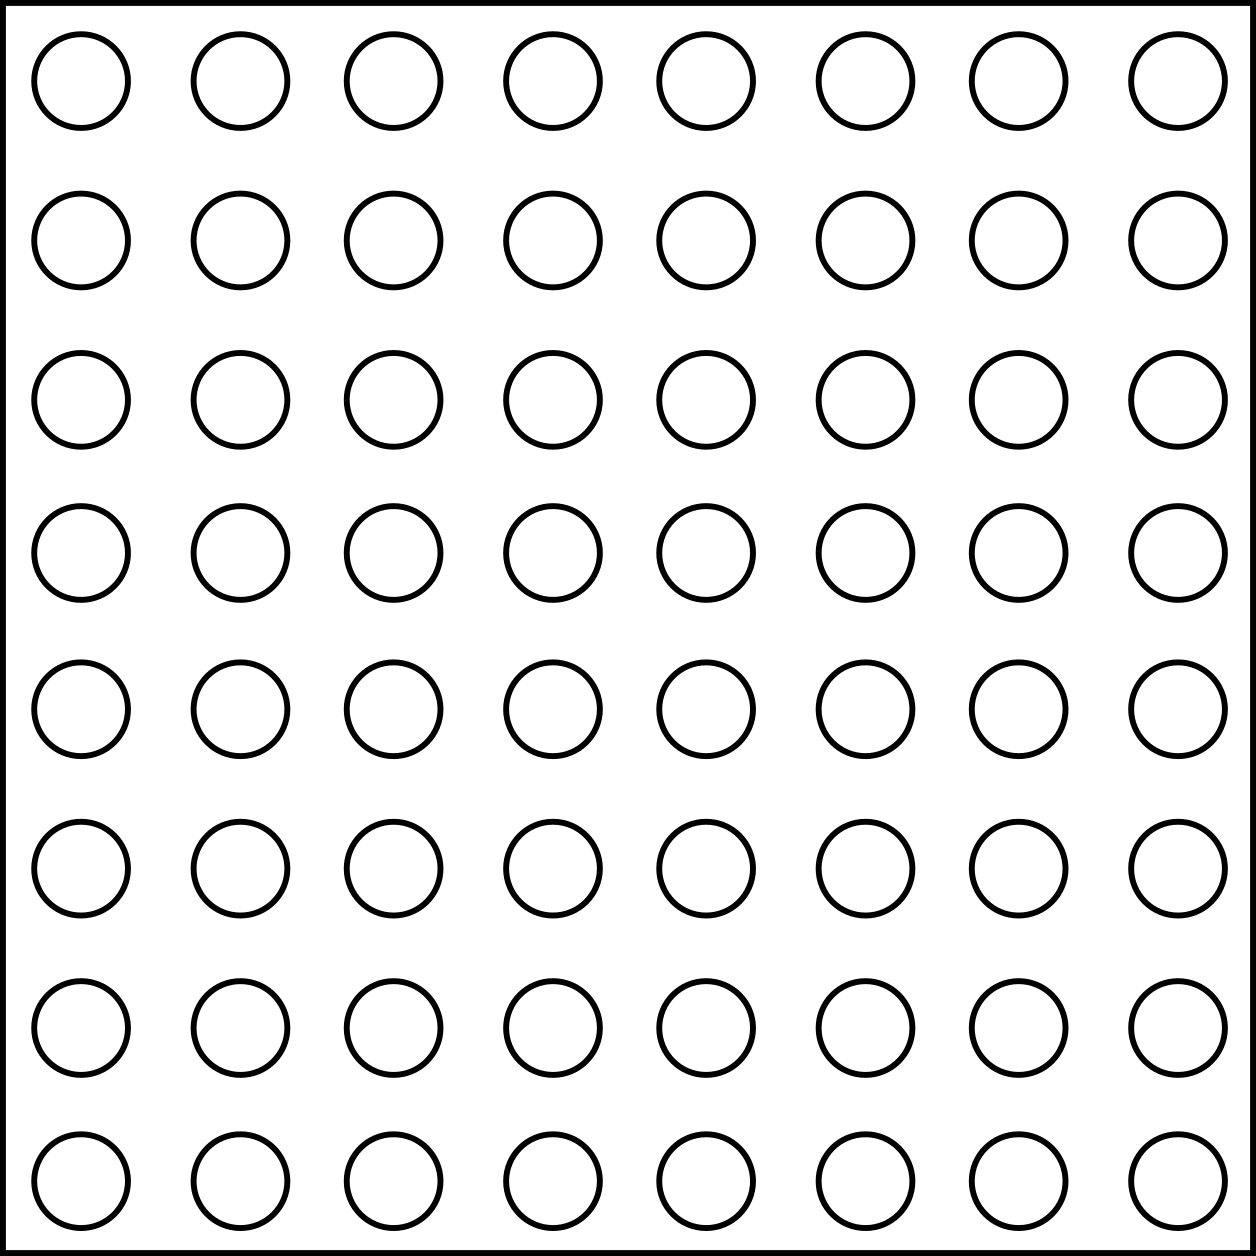
\includegraphics[width=0.80\textwidth]{cnn_neurones.png}

      \end{center}
    \end{column}

    \begin{column}<3->{0.33\textwidth}
      \begin{center}
        
\includegraphics[width=0.07\textwidth]{col.png}

      \end{center}
    \end{column}

  \end{columns}


\end{frame}


%%%%%%%%%%%%%%%%%%%%%%%%%%%%%%%%%%%%%%%%%%%%%%%%%%
\frame{
  \frametitle{Towards convolutional layers}


  \begin{columns}

    \begin{column}<1->{0.3\textwidth}
      \begin{center}
        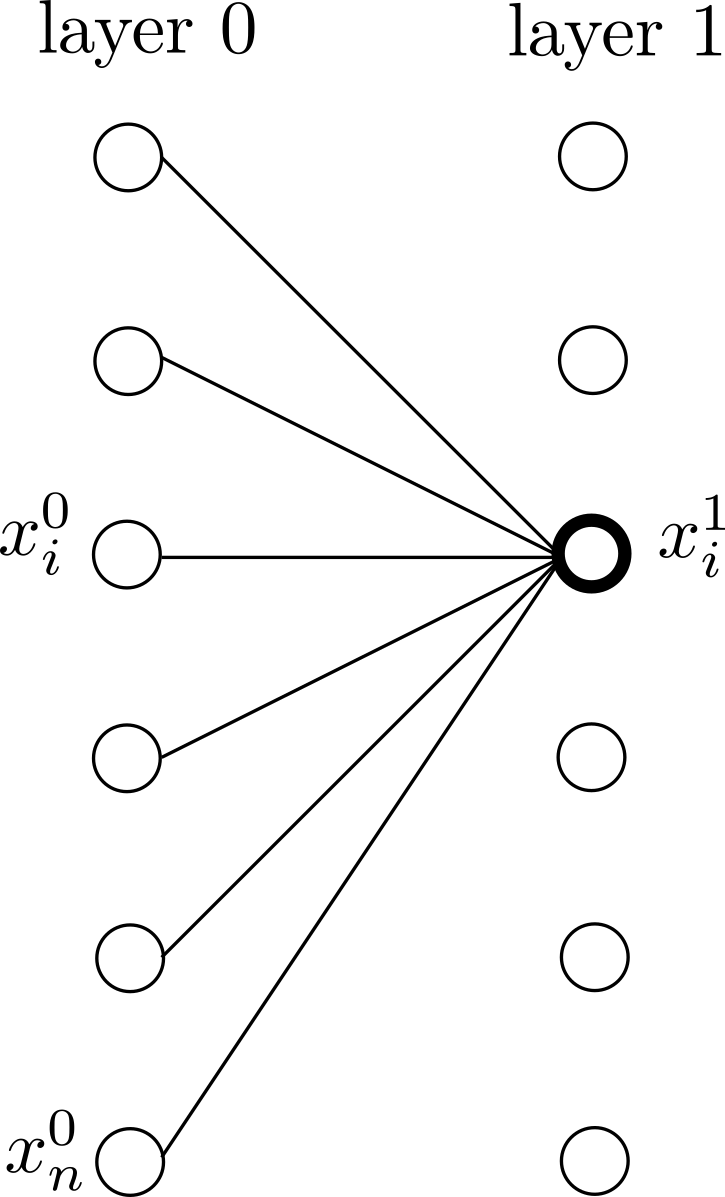
\includegraphics[width=0.74\textwidth]{fully_connected_layer.png}
        \\ \scriptsize{Fully connected layer: $n(n+1)$ weights}
      \end{center}
    \end{column}

    \begin{column}<2->{0.3\textwidth}
      \begin{center}
        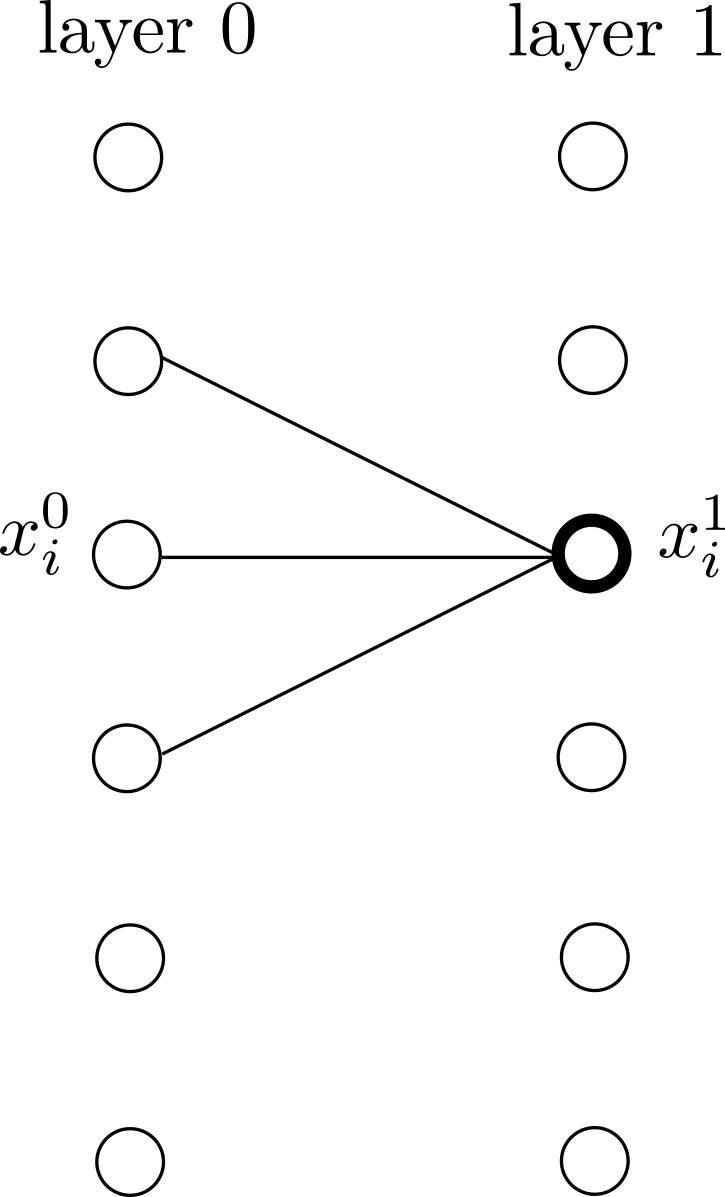
\includegraphics[width=0.74\textwidth]{locally_connected_layer.png}
        \\ \scriptsize{Locally conn. layer: $n(s+1)$ weights}
      \end{center}
    \end{column}

    \begin{column}<3->{0.3\textwidth}
      \begin{center}
        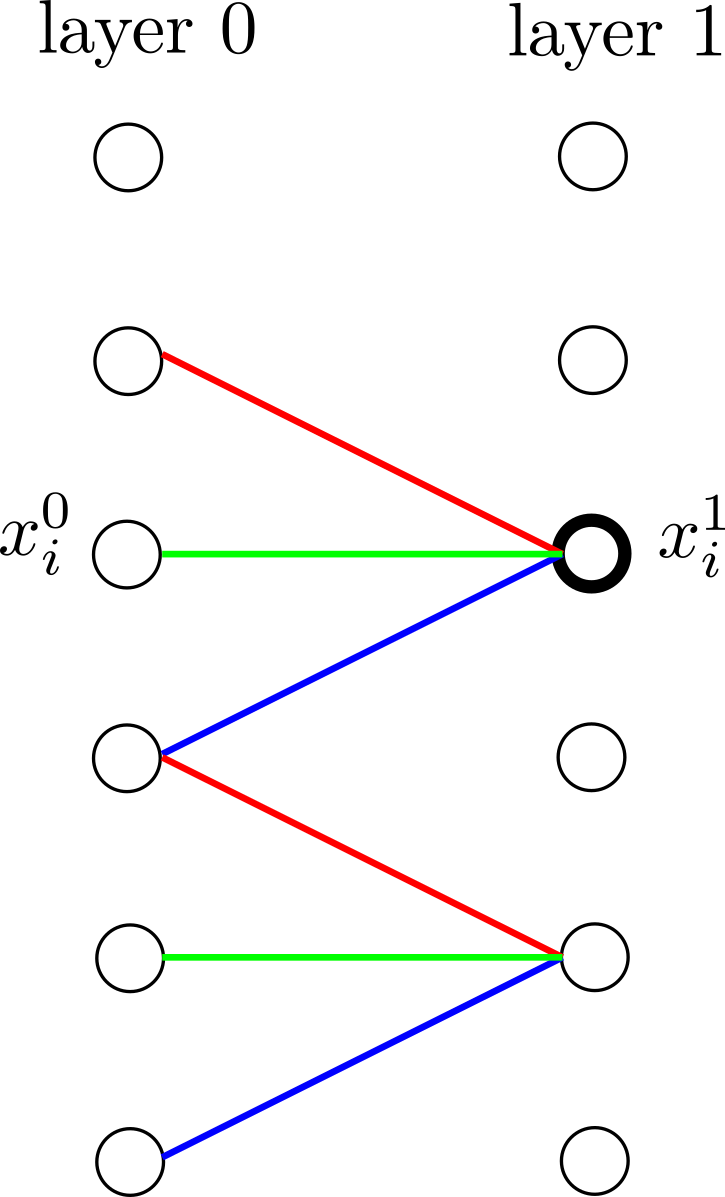
\includegraphics[width=0.74\textwidth]{convolutional_layer.png}
        \\ \scriptsize{Weight replication: $s+1$ weights.\\
          \alert{Convolutional layer.}}
      \end{center}
    \end{column}

  \end{columns}

}


%%%%%%%%%%%%%%%%%%%%%%%%%%%%%%%%%%%%%%%%%%%%%%%%%%
\frame{
  \frametitle{Towards convolutional layers: some figures}

  \begin{itemize}
  \item $3 \times 3$ convolutions: $s=9$
  \item \textcolor{blue}{Toy image: $n = 28 \times 28 = 784$}
  \item \textcolor{orange}{Typical image: $n = 1000 \times 1000 = 10^6$}
  \end{itemize}

  \begin{columns}

    \begin{column}{0.3\textwidth}
      \begin{center}
        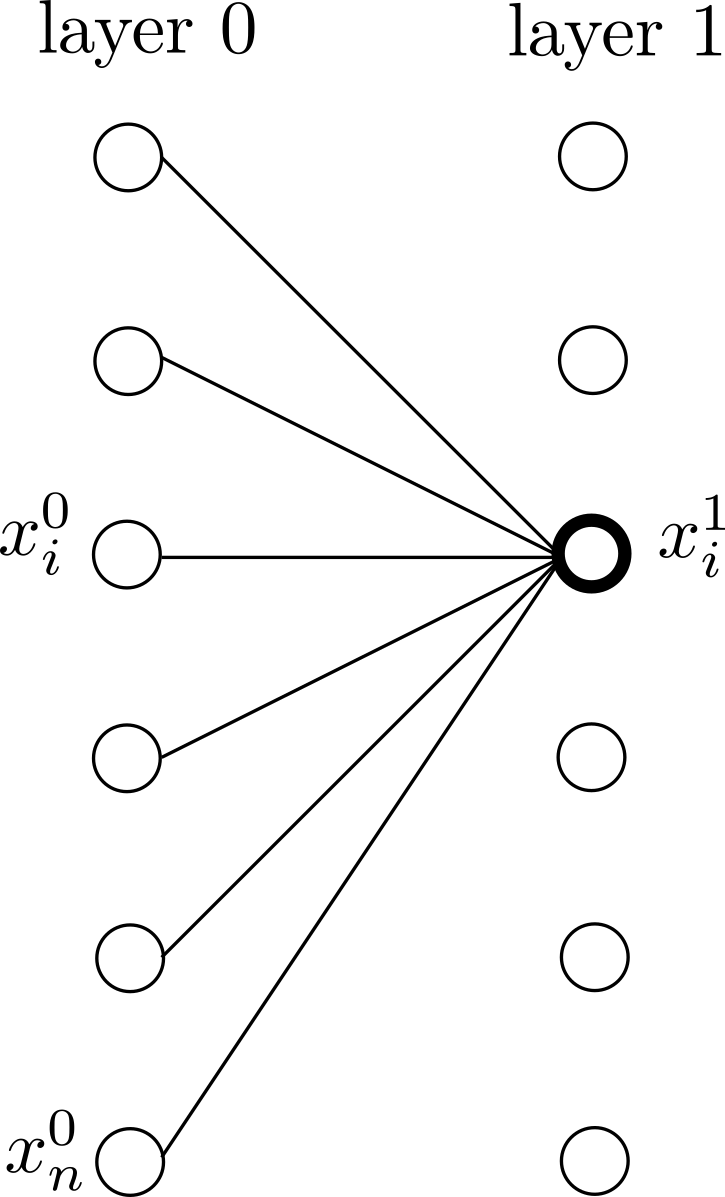
\includegraphics[width=0.74\textwidth]{fully_connected_layer.png}
        \\ \scriptsize{Fully connected layer: $n(n+1)$ weights}
        \\ \textcolor{blue}{\scriptsize{$\approx 6.10^5$}}
        \\ \textcolor{orange}{\scriptsize{$\approx 10^{12}$}}
      \end{center}
    \end{column}

    \begin{column}{0.3\textwidth}
      \begin{center}
        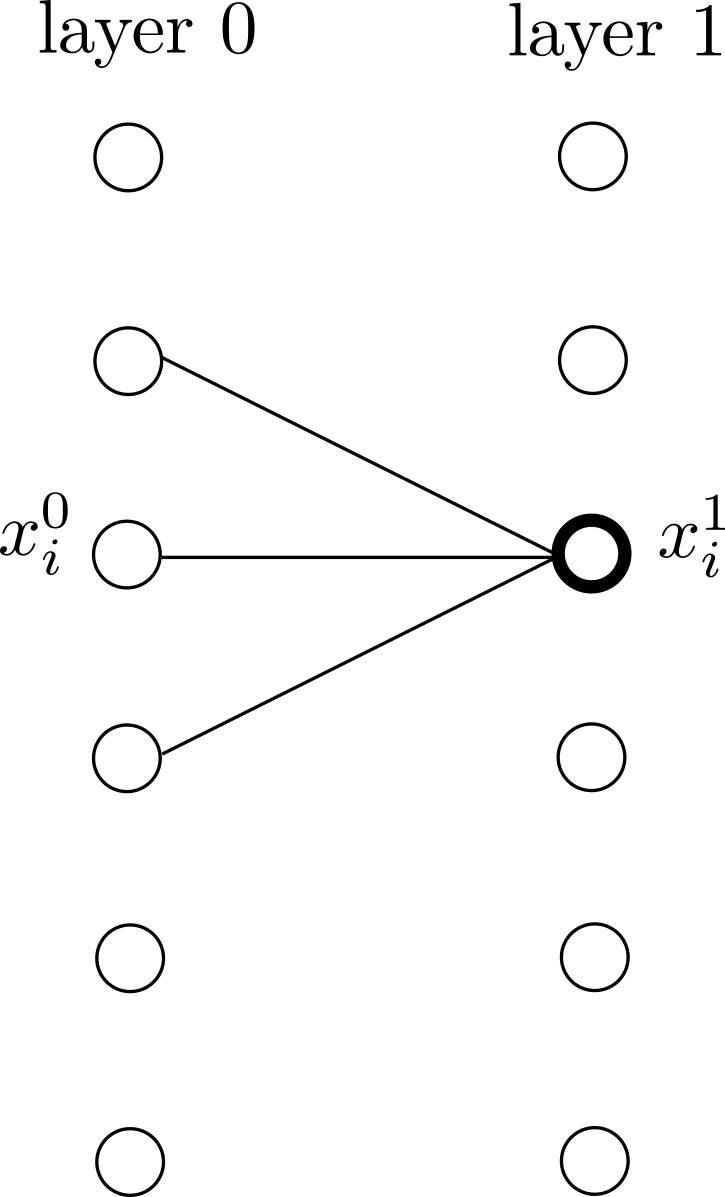
\includegraphics[width=0.74\textwidth]{locally_connected_layer.png}
        \\ \scriptsize{Locally conn. layer: $n(s+1)$ weights}
        \\ \textcolor{blue}{\scriptsize{$7840$}}
        \\ \textcolor{orange}{\scriptsize{$10^7$}}
      \end{center}
    \end{column}

    \begin{column}{0.3\textwidth}
      \begin{center}
        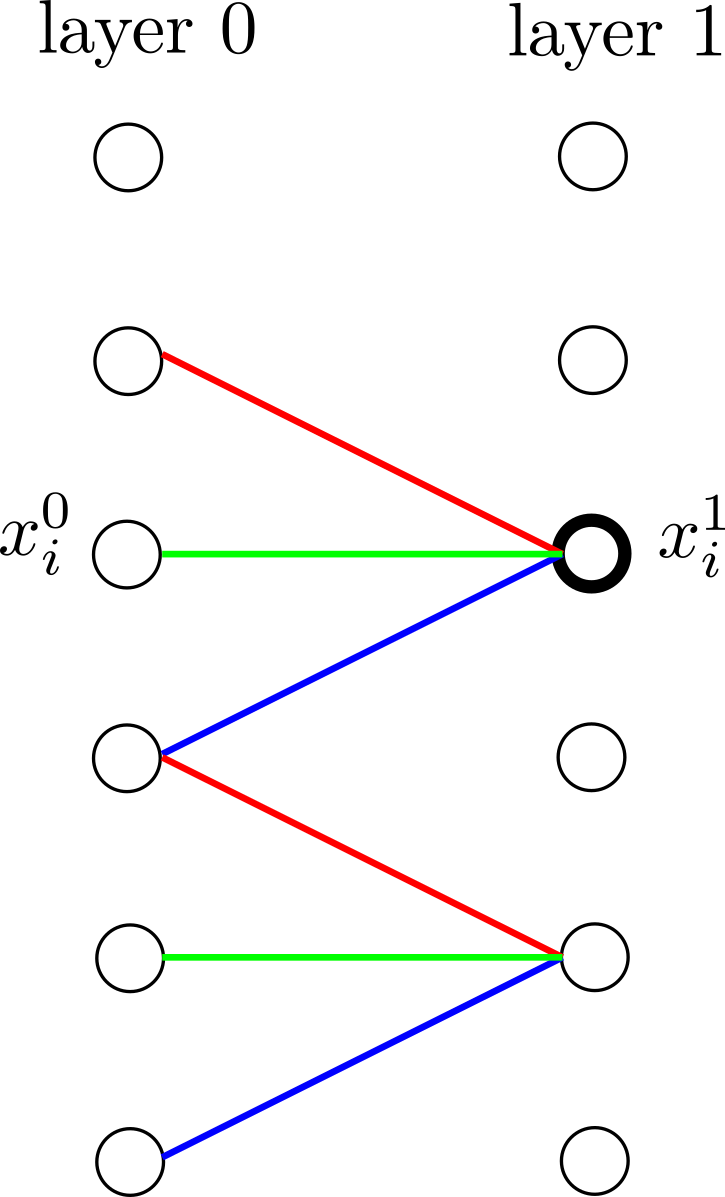
\includegraphics[width=0.74\textwidth]{convolutional_layer.png}
        \\ \scriptsize{Weight replication: $s+1$ weights.}
        \\ \textcolor{blue}{\scriptsize{$10$}}
        \\ \textcolor{orange}{\scriptsize{$10$}}

      \end{center}
    \end{column}

  \end{columns}
}


%%%%%%%%%%%%%%%%%%%%%%%%%%%%%%%%%%%%
\begin{frame}{Convolutional layer illustration in 2D}


  \begin{itemize}
  \item Illustration of a convolution of size $3 \times 3$
  \end{itemize}

  \begin{center}
    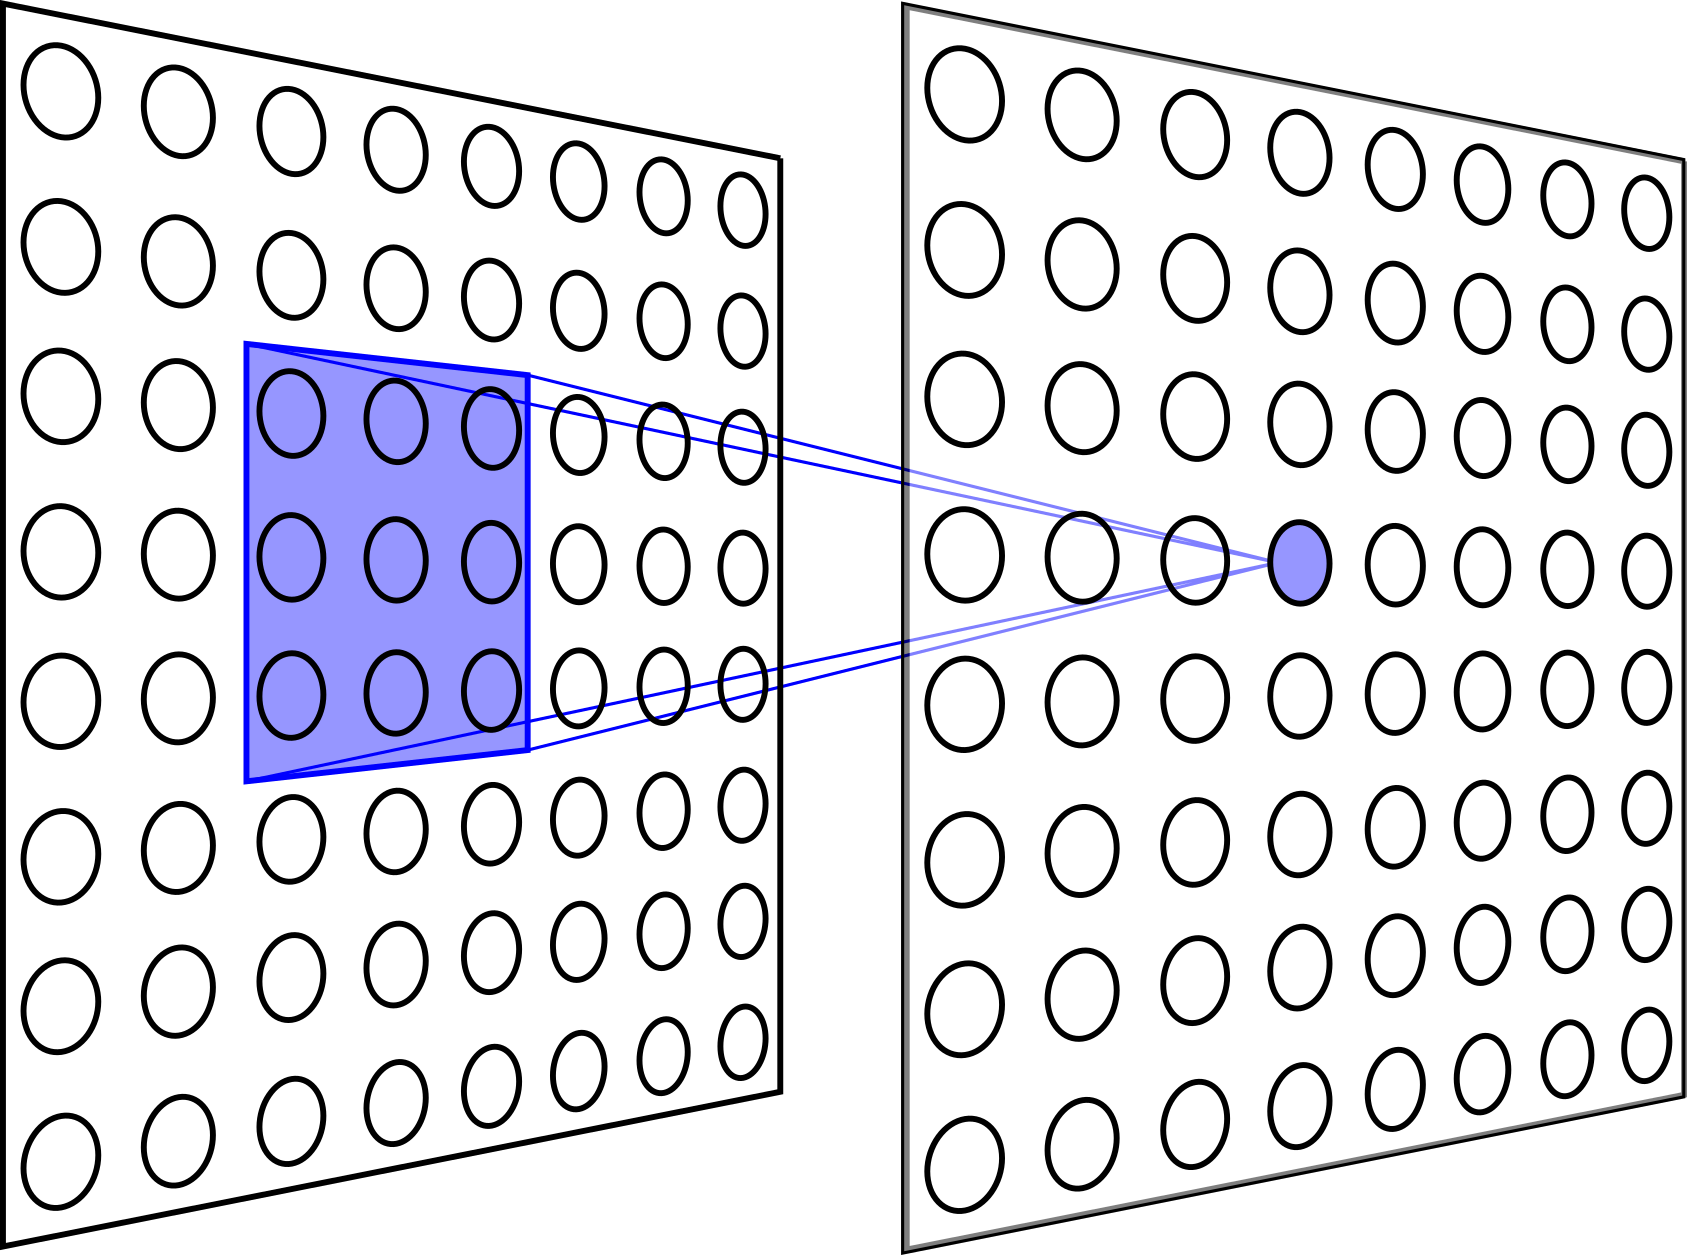
\includegraphics[width=0.5\textwidth]{cnn_complet}
  \end{center}


\end{frame}

%%%%%%%%%%%%%%%%%%%%%%%%%%%%%%%%%%%%
\begin{frame}{1D representations}

  \centering
  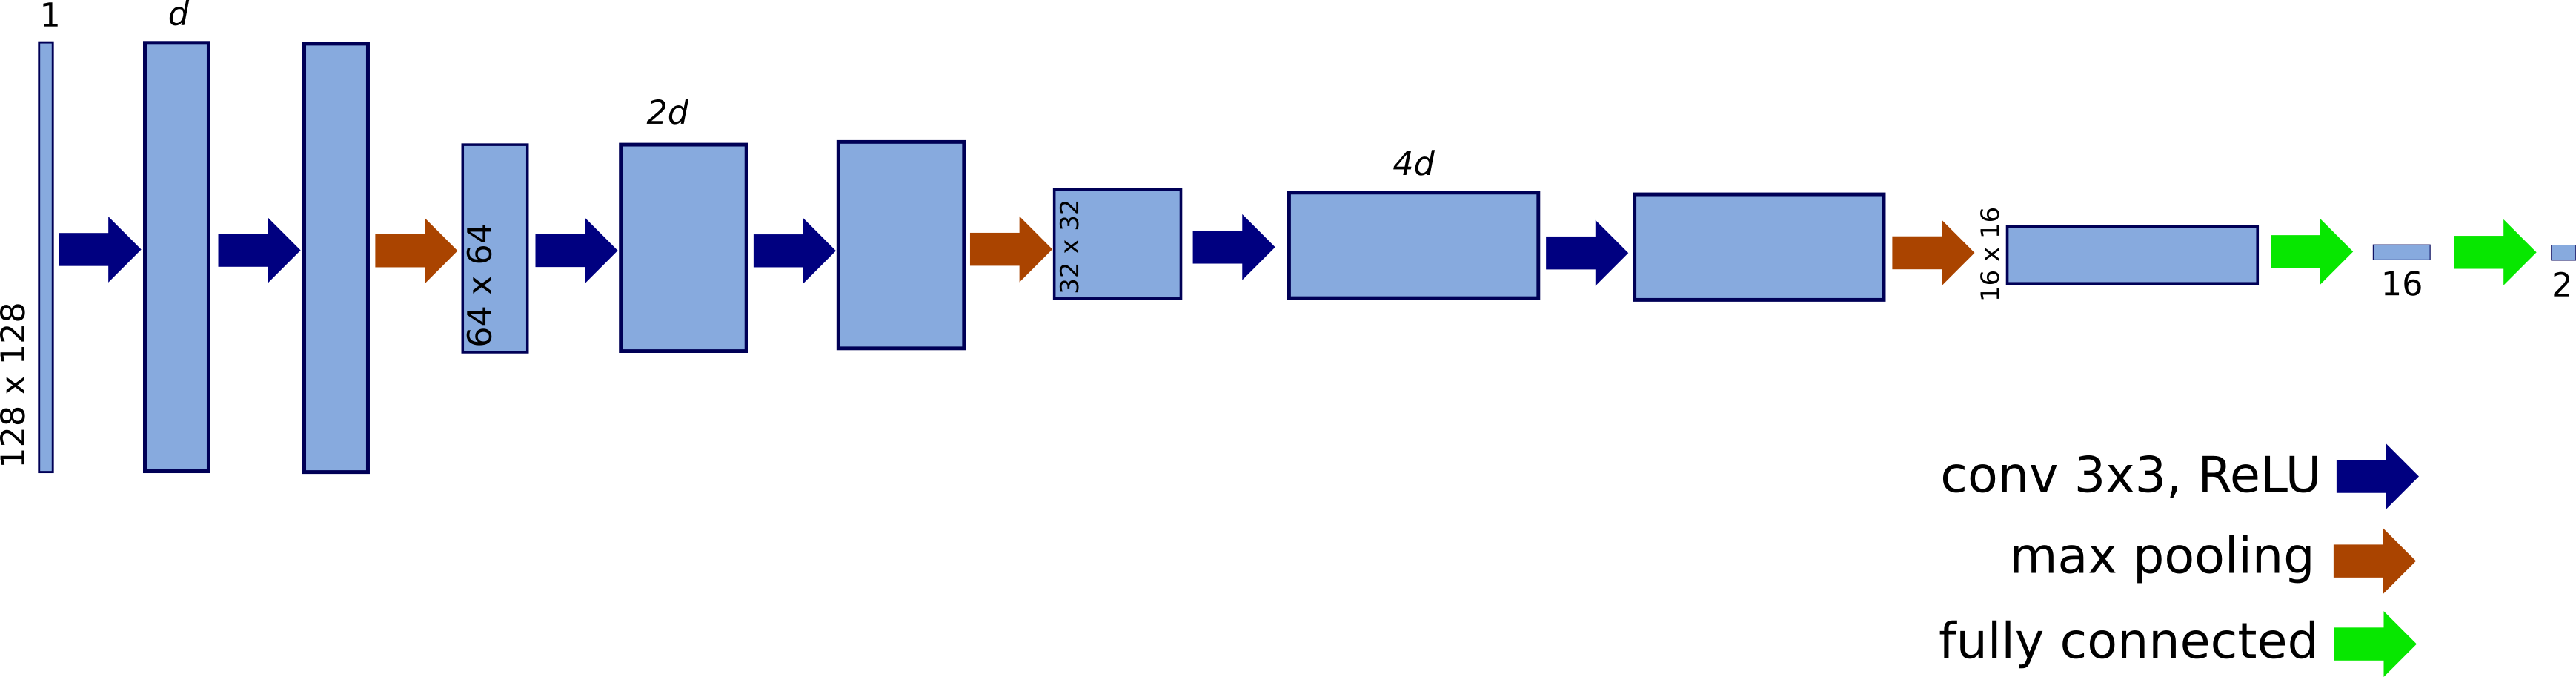
\includegraphics[width=\textwidth]{fovea_convnet2}

  \vspace{1em}
  \pause

  \begin{columns}
    \begin{column}{.5\textwidth}
      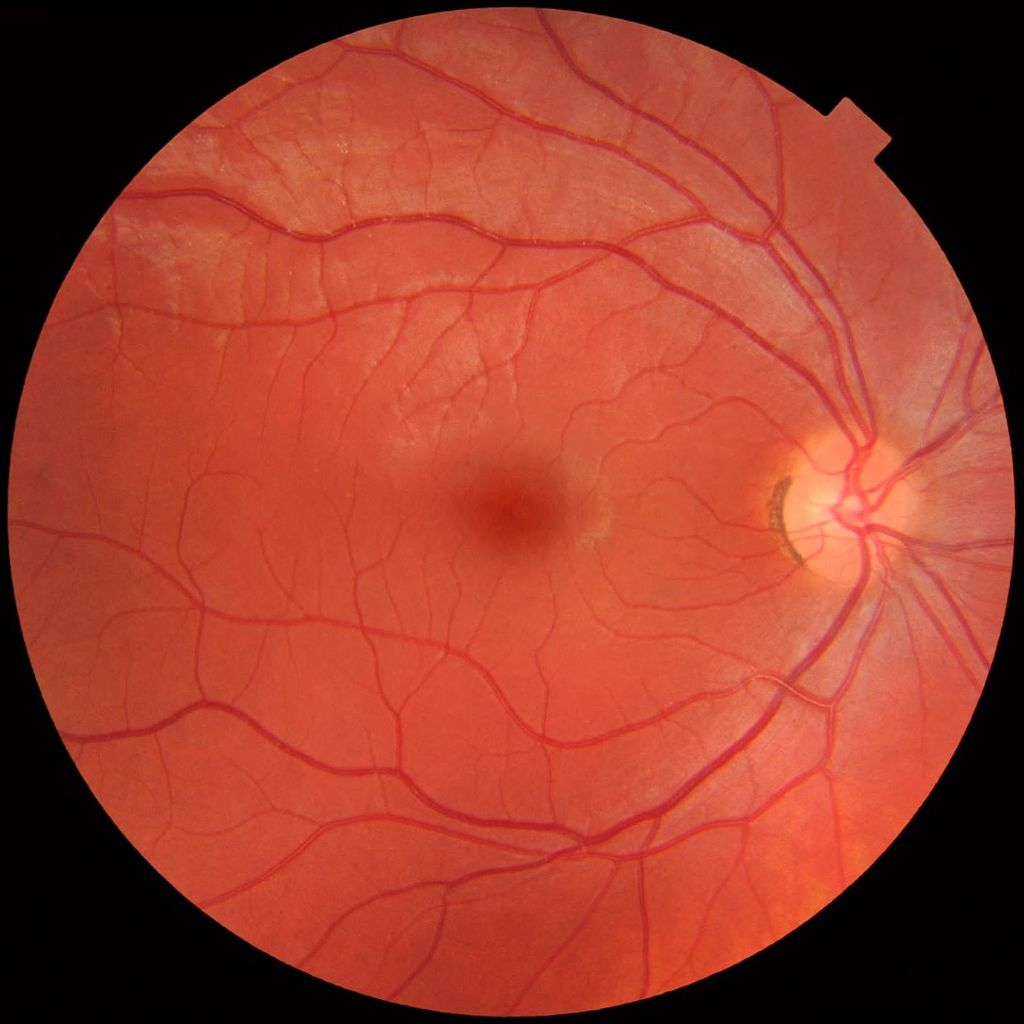
\includegraphics[width=0.8\textwidth]{Fundus_photograph_of_normal_right_eye.jpg}
    \end{column}
    \begin{column}{.5\textwidth}
      This NN was used to estimate the position of the center of the macula on fundus images.
    \end{column}
  \end{columns}

  \source{NN is work of Robin Alais et al.\\Fundus image by Mikael Häggström, used with permission (CC0).}


\end{frame}


%%%%%%%%%%%%%%%%%%%%%%%%%%%%%%%%%%%%%%%%%%%%%%%%%%
\frame{
  \frametitle{U-Net architecture \cite{ronneberger_u-net:_2015}}

  \begin{figure}
    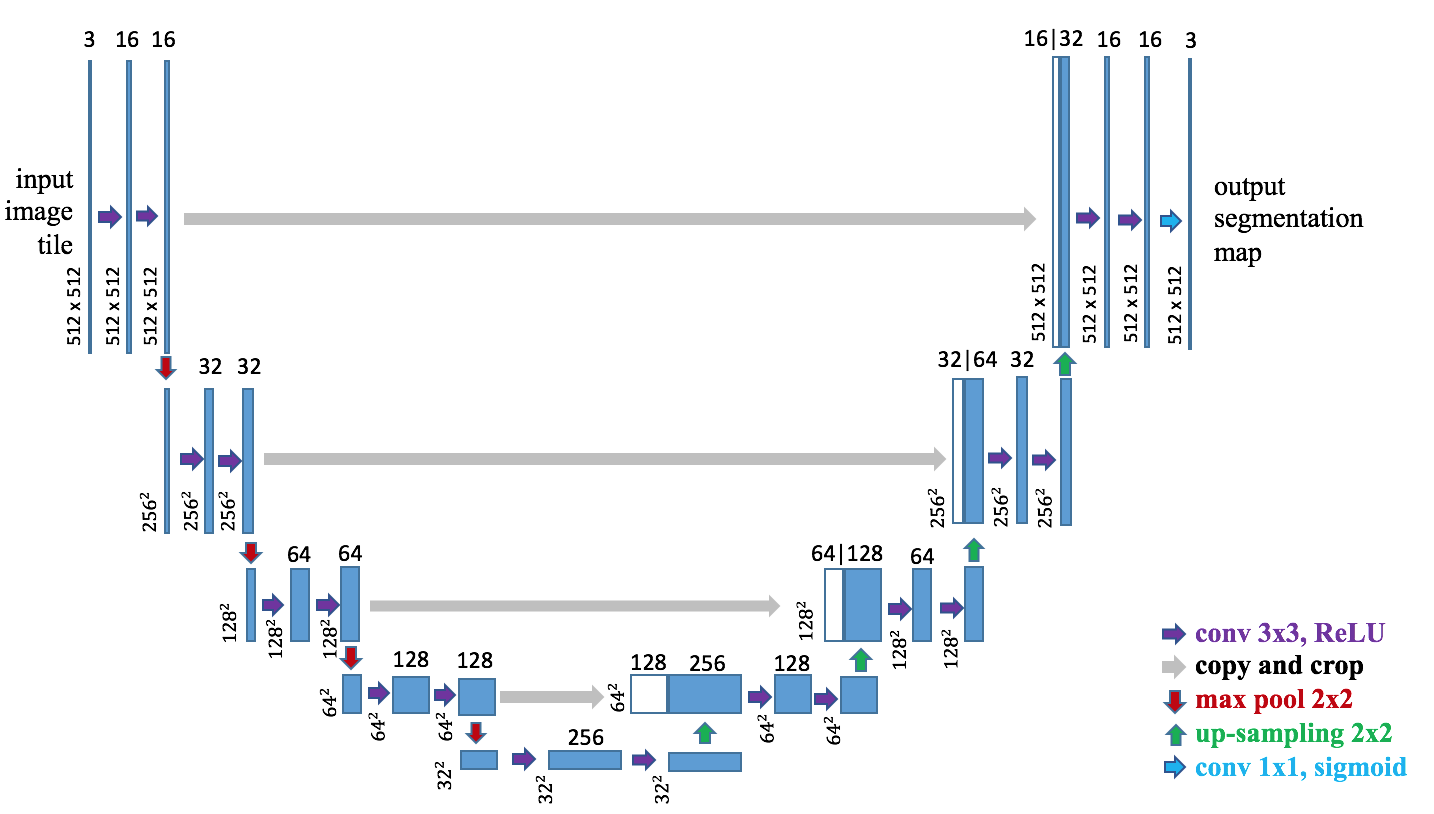
\includegraphics[width=0.95\textwidth]{unet_lo}
  \end{figure}

}



%%%%%%%%%%%%%%%%%%%%%%%%%%%%%%%%%%%%
\begin{frame}{Example: counting cells}

    \begin{figure}
      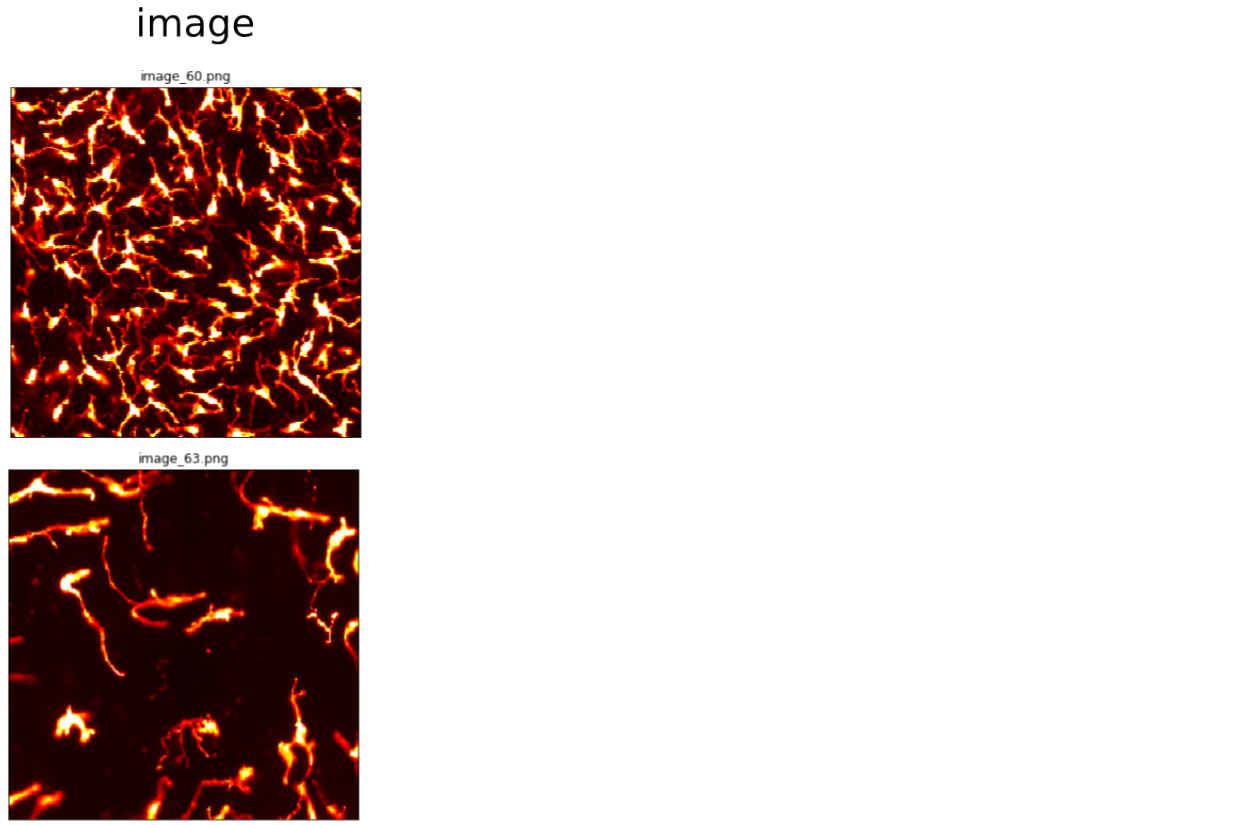
\includegraphics[width=\textwidth]{lazard0}
      \source{Tristan Lazard, master thesis. In collaboration with L'Oréal.}
    \end{figure}

\end{frame}


%%%%%%%%%%%%%%%%%%%%%%%%%%%%%%%%%%%%
\begin{frame}{Counting cells}

    \begin{figure}
      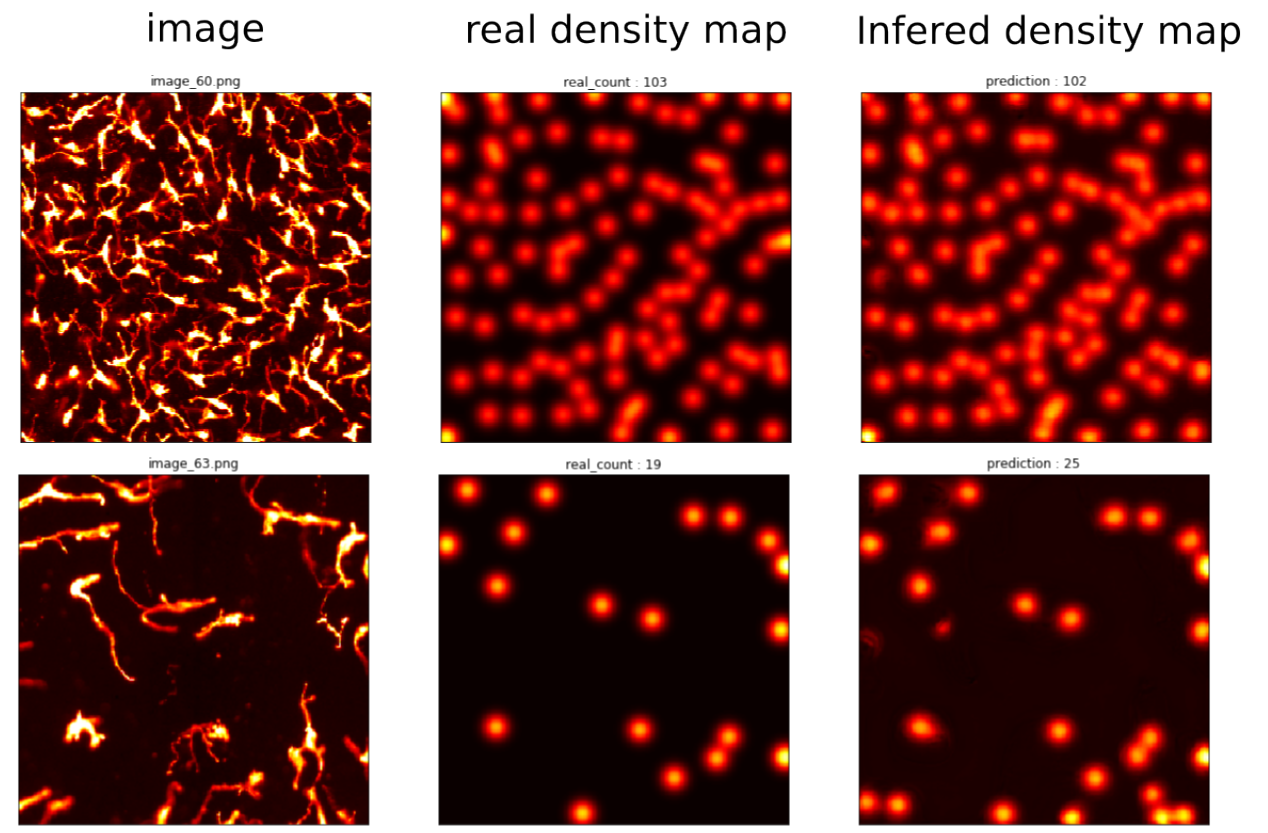
\includegraphics[width=\textwidth]{lazard}
      \source{Tristan Lazard, master thesis. In collaboration with L'Oréal.}
    \end{figure}

\end{frame}

%%%%%%%%%%%%%%%%%%%%%%%%%%%%%%%%%%
\section{Autoencoders and generative adversarial networks}
%%%%%%%%%%%%%%%%%%%%%%%%%%%%%%%%%%

%%%%%%%%%%%%%%%%%%%%%%%%%%%%%%%%%%
\begin{frame}%{Reminder of Machine Learning Problems}
  {Supervised Learning}

  Given a labeled dataset $(\X,\mathbf{Y})$, we would like to learn a mapping from data space to label space.
\begin{figure}
\centering
\begin{tikzpicture}
\tikzstyle{main}=[circle, minimum size = 6mm, thick, draw =black!80, node distance = 26mm]
\tikzstyle{connect}=[-latex, thick]
  \node[main, fill = white!50] (alpha) [label=below: $\x$] {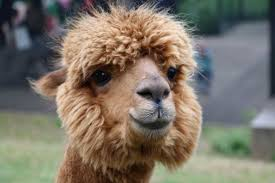
\includegraphics[width=.15\columnwidth]{Animal}};
  \node[main,fill = red!50] (xout) [right= of alpha,label=below: What animal is this?] {$\hat{\y} \in \mathbb{Z}$ };
  \draw[thick,->] (alpha) -- (xout) node[midway,sloped,above] {Classification};
  \end{tikzpicture}
\end{figure}
%% \begin{figure}
%% \centering
%% \begin{tikzpicture}
%% \tikzstyle{main}=[circle, minimum size = 6mm, thick, draw =black!80, node distance = 26mm]
%% \tikzstyle{connect}=[-latex, thick]
%%   \node[main, fill = white!50] (alpha) [label=below: $\x$] {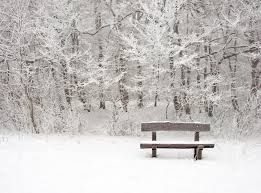
\includegraphics[width=.15\columnwidth]{Winter}};
%%   \node[main,fill = red!50] (xout) [right= of alpha,label=below: How cold is it?] {$\hat{\y} \in \mathbb{R}$ };
%%   \draw[thick,->] (alpha) -- (xout) node[midway,sloped,above] {Regression};
%%   \end{tikzpicture}
%% \end{figure}
\end{frame}


%% \begin{frame}{Unsupervised Learning: Clustering}
%% Given an unlabeled dataset $(\X)$, we would like to learn:
%% \alert{How to group objects into categories?}
%% \begin{figure}
%% \centering
%% \begin{tikzpicture}
%% \tikzstyle{main}=[circle, minimum size = 9mm, thick, draw =black!80, node distance = 26mm]
%% \tikzstyle{connect}=[-latex, thick]
%%   \node[main, fill = white!50] (alpha) [label=below: $\X$ ] {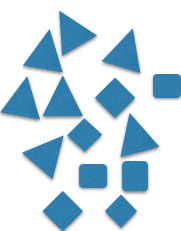
\includegraphics[width=.2\columnwidth]{Shapes}};
%%   \node[main,fill = white!50] (xout) [right= of alpha,label=below: $\hat{\mathbf{Y}} \in \mathbb{Z}$] {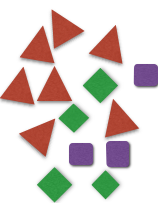
\includegraphics[width=.2\columnwidth]{ShapesClusters}};
%%   \draw[thick,->] (alpha) -- (xout) node[midway,sloped,above] {Clustering};
%%   \end{tikzpicture}
%% \end{figure}
%% \end{frame}

%% \begin{frame}{Unsupervised Learning: Anomaly detection}
%% Given an unlabeled dataset $(\X)$, we would like to learn:
%% \alert{How to identify observations differing significantly from the majority of data?}
%% \begin{figure}
%% \centering
%% \begin{tikzpicture}
%% \tikzstyle{main}=[circle, minimum size = 9mm, thick, draw =black!80, node distance = 30mm]
%% \tikzstyle{connect}=[-latex, thick]
%%   \node[main, fill = white!50] (alpha) [label=below: $\X$ ] {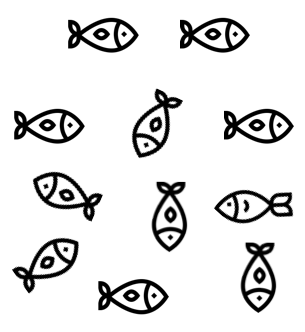
\includegraphics[width=.2\columnwidth]{Anomaly1}};
%%   \node[main,fill = white!50] (xout) [right= of alpha,label=below: $\hat{\mathbf{Y}} \in \{\mathbf{0,1}\}$] {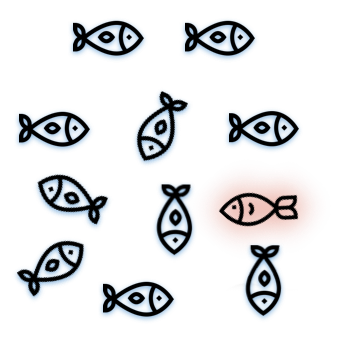
\includegraphics[width=.2\columnwidth]{Anomaly2}};
%%   \draw[thick,->] (alpha) -- (xout) node[midway,sloped,above] {Anomaly Detection};
%%   \end{tikzpicture}
%% \end{figure}
%% \end{frame}


\begin{frame}{Autoencoders}

\begin{figure}
\centering
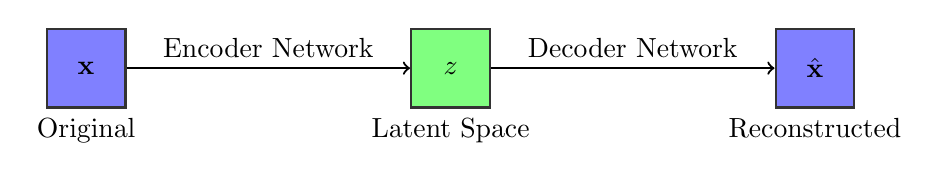
\begin{tikzpicture}
\tikzstyle{main}=[rectangle, minimum size = 10mm, thick, draw =black!80, node distance = 36mm]
\tikzstyle{connect}=[-latex, thick]
  \node[main, fill = blue!50] (alpha) [label=below: Original ] {$\x$};
  \node[main,fill = green!50] (z) [right=of alpha,label=below:Latent Space] { $z$};
  \node[main,fill = blue!50] (xout) [right= of z,label=below: Reconstructed ] {$\hat{\x}$ };
  \draw[thick,->] (alpha) -- (z) node[midway,sloped,above] {Encoder Network};
  \draw[thick,->] (z) -- (xout) node[midway,sloped,above] {Decoder Network};
  \end{tikzpicture}
\end{figure}

\end{frame}



\begin{frame}{Unsupervised learning: Generative Models}
  Given an unlabeled dataset $(\X)$, we would like to learn:
\alert{How to generate a new observation from the same distribution (unknown) of dataset?}
\begin{figure}
\centering
\begin{tikzpicture}
\tikzstyle{main}=[circle, minimum size = 9mm, thick, draw =black!80, node distance = 30mm]
\tikzstyle{connect}=[-latex, thick]
  \node[main, fill = white!50] (alpha) [label=below: $\X$ ] {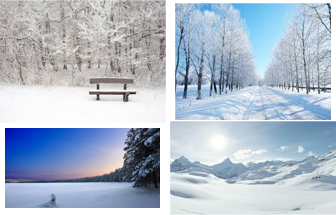
\includegraphics[width=.2\columnwidth]{Generative1}};
  \node[main,fill = white!50] (xout) [right= of alpha,label=below: $\mathbf{x}_{\texttt{new}}$] {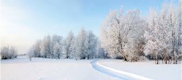
\includegraphics[width=.2\columnwidth]{Generative2}};
  \draw[thick,->] (alpha) -- (xout) node[midway,sloped,above] {Generative model};
  \end{tikzpicture}
\end{figure}
\end{frame}



%%%%%%%%%%%%%%%%%%%%%%%%%%%%%%%%%%%%
\begin{frame}{Generative adversarial networks \cite{goodfellow_generative_2014}}

  \begin{figure}[ht]
    \centering
    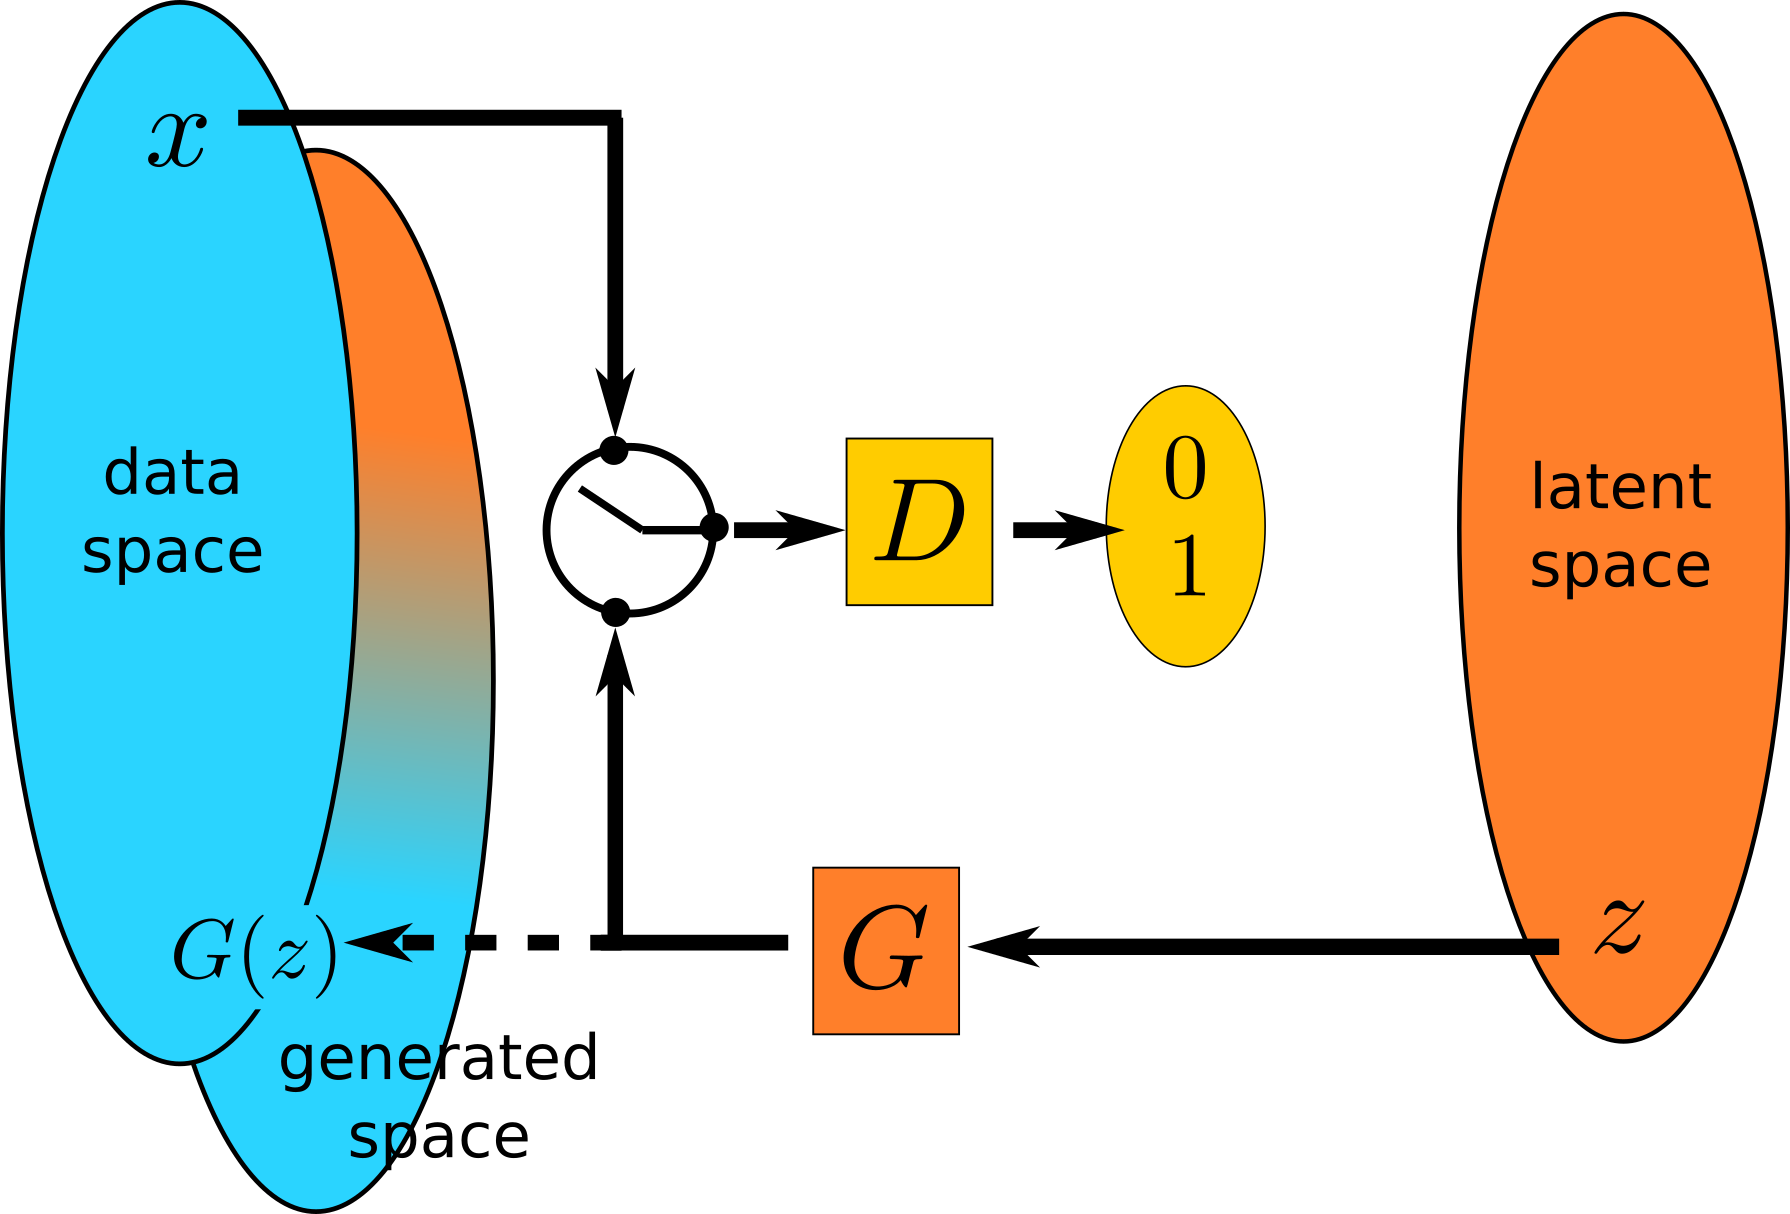
\includegraphics[width=0.5\textwidth]{gan2}
  \end{figure}

  \begin{itemize}
  \item The \alert{discriminator} $D$ is optimized so that it correctly classifies images as real (1) or fake (0)
  \item The \alert{generator} $G$ is optimized so that the produced images are classified as real by the discriminator
  \end{itemize}

\end{frame}

%%%%%%%%%%%%%%%%%%%%%%%%%%%%%%%%%%%%
\begin{frame}{Which face is real?}

  \url{https://www.whichfaceisreal.com/}

\end{frame}


%%%%%%%%%%%%%%%%%%%%%%%%%%%%%%%%%%
\section{Conclusion}

%%%%%%%%%%%%%%%%%%%%%%%%%%%%%%%%%%%%
\begin{frame}{Conclusion}

\begin{itemize}
\item Deep learning allows to learn complex transformations between tensors, thanks to:
  \begin{itemize}
  \item Smart methods and algorithms.
  \item Lots of annotated data.
  \item Specialized hardware (for learning).
  \end{itemize}
\item Drawbacks:
  \begin{itemize}
  \item Interpretability problem.
  \item Why does deep learning work so well?
  \item Deep learning can be easily fooled.
  \end{itemize}
  \item General artificial intelligence is still far away
\end{itemize}

\end{frame}



%%%%%%%%%%%%%%%%%%%%%%%%%%%%%%%%%%%%%%%%%%%%%%%%%%

\frame{
  \frametitle{ConvNets can be fooled \tiny\cite{nguyen_deep_2015}}

  \begin{figure}
    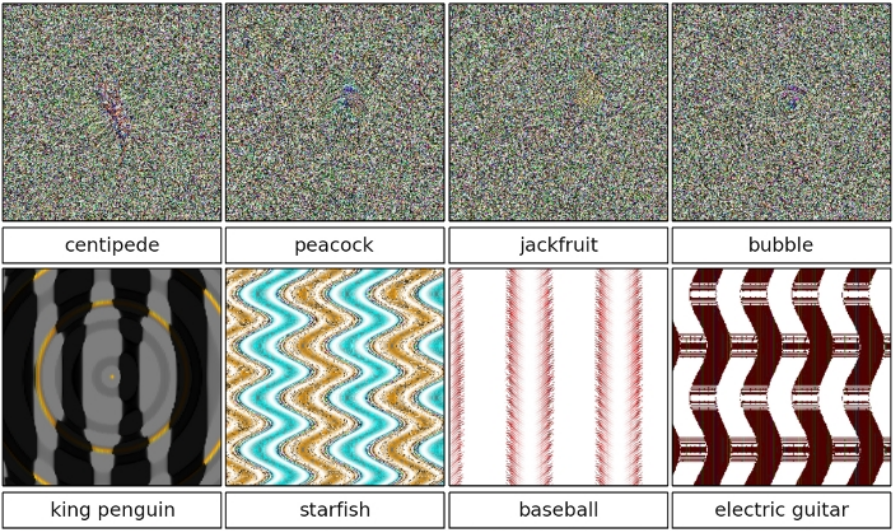
\includegraphics[width=0.9\textwidth]{dl_easily_fooled.png}
  \end{figure}


}



%%%%%%%%%%%%%%%%%%%%%%%%%%%%%%%%%%%%%%%%%%%%%%%%%%
\section*{References}

%%%%%%%%%%%%%%%%%%%%%%%%%%%%%%%%%%%%%%%%%%%%%%%%%%

\frame[allowframebreaks]{

  \scriptsize

  \frametitle{References}

  %\bibliographystyle{amsalpha}
  %\bibliographystyle{apalike}

  \bibliography{../../edf.bib,slides_deep.bib}

  \normalsize

}



\end{document}
